\documentclass[twoside]{book}

% Packages required by doxygen
\usepackage{fixltx2e}
\usepackage{calc}
\usepackage{doxygen}
\usepackage[export]{adjustbox} % also loads graphicx
\usepackage{graphicx}
\usepackage[utf8]{inputenc}
\usepackage{makeidx}
\usepackage{multicol}
\usepackage{multirow}
\PassOptionsToPackage{warn}{textcomp}
\usepackage{textcomp}
\usepackage[nointegrals]{wasysym}
\usepackage[table]{xcolor}

% Font selection
\usepackage[T1]{fontenc}
\usepackage[scaled=.90]{helvet}
\usepackage{courier}
\usepackage{amssymb}
\usepackage{sectsty}
\renewcommand{\familydefault}{\sfdefault}
\allsectionsfont{%
  \fontseries{bc}\selectfont%
  \color{darkgray}%
}
\renewcommand{\DoxyLabelFont}{%
  \fontseries{bc}\selectfont%
  \color{darkgray}%
}
\newcommand{\+}{\discretionary{\mbox{\scriptsize$\hookleftarrow$}}{}{}}

% Page & text layout
\usepackage{geometry}
\geometry{%
  a4paper,%
  top=2.5cm,%
  bottom=2.5cm,%
  left=2.5cm,%
  right=2.5cm%
}
\tolerance=750
\hfuzz=15pt
\hbadness=750
\setlength{\emergencystretch}{15pt}
\setlength{\parindent}{0cm}
\setlength{\parskip}{3ex plus 2ex minus 2ex}
\makeatletter
\renewcommand{\paragraph}{%
  \@startsection{paragraph}{4}{0ex}{-1.0ex}{1.0ex}{%
    \normalfont\normalsize\bfseries\SS@parafont%
  }%
}
\renewcommand{\subparagraph}{%
  \@startsection{subparagraph}{5}{0ex}{-1.0ex}{1.0ex}{%
    \normalfont\normalsize\bfseries\SS@subparafont%
  }%
}
\makeatother

% Headers & footers
\usepackage{fancyhdr}
\pagestyle{fancyplain}
\fancyhead[LE]{\fancyplain{}{\bfseries\thepage}}
\fancyhead[CE]{\fancyplain{}{}}
\fancyhead[RE]{\fancyplain{}{\bfseries\leftmark}}
\fancyhead[LO]{\fancyplain{}{\bfseries\rightmark}}
\fancyhead[CO]{\fancyplain{}{}}
\fancyhead[RO]{\fancyplain{}{\bfseries\thepage}}
\fancyfoot[LE]{\fancyplain{}{}}
\fancyfoot[CE]{\fancyplain{}{}}
\fancyfoot[RE]{\fancyplain{}{\bfseries\scriptsize Generated by Doxygen }}
\fancyfoot[LO]{\fancyplain{}{\bfseries\scriptsize Generated by Doxygen }}
\fancyfoot[CO]{\fancyplain{}{}}
\fancyfoot[RO]{\fancyplain{}{}}
\renewcommand{\footrulewidth}{0.4pt}
\renewcommand{\chaptermark}[1]{%
  \markboth{#1}{}%
}
\renewcommand{\sectionmark}[1]{%
  \markright{\thesection\ #1}%
}

% Indices & bibliography
\usepackage{natbib}
\usepackage[titles]{tocloft}
\setcounter{tocdepth}{3}
\setcounter{secnumdepth}{5}
\makeindex

% Hyperlinks (required, but should be loaded last)
\usepackage{ifpdf}
\ifpdf
  \usepackage[pdftex,pagebackref=true]{hyperref}
\else
  \usepackage[ps2pdf,pagebackref=true]{hyperref}
\fi
\hypersetup{%
  colorlinks=true,%
  linkcolor=blue,%
  citecolor=blue,%
  unicode%
}

% Custom commands
\newcommand{\clearemptydoublepage}{%
  \newpage{\pagestyle{empty}\cleardoublepage}%
}

\usepackage{caption}
\captionsetup{labelsep=space,justification=centering,font={bf},singlelinecheck=off,skip=4pt,position=top}

%===== C O N T E N T S =====

\begin{document}

% Titlepage & ToC
\hypersetup{pageanchor=false,
             bookmarksnumbered=true,
             pdfencoding=unicode
            }
\pagenumbering{alph}
\begin{titlepage}
\vspace*{7cm}
\begin{center}%
{\Large termschem }\\
\vspace*{1cm}
{\large Generated by Doxygen 1.8.13}\\
\end{center}
\end{titlepage}
\clearemptydoublepage
\pagenumbering{roman}
\tableofcontents
\clearemptydoublepage
\pagenumbering{arabic}
\hypersetup{pageanchor=true}

%--- Begin generated contents ---
\chapter{Bug List}
\label{bug}
\Hypertarget{bug}

\begin{DoxyRefList}
\item[\label{bug__bug000001}%
\Hypertarget{bug__bug000001}%
File \hyperlink{arrayhelper_8h}{arrayhelper.h} ]No known bugs.  
\item[\label{bug__bug000002}%
\Hypertarget{bug__bug000002}%
File \hyperlink{mtxhelper_8h}{mtxhelper.h} ]No known bugs. 
\end{DoxyRefList}
\chapter{File Index}
\section{File List}
Here is a list of all files with brief descriptions\+:\begin{DoxyCompactList}
\item\contentsline{section}{include/\hyperlink{arrayhelper_8h}{arrayhelper.\+h} \\*A set of macros that help manage arrays }{\pageref{arrayhelper_8h}}{}
\item\contentsline{section}{include/\hyperlink{charhelper_8h}{charhelper.\+h} }{\pageref{charhelper_8h}}{}
\item\contentsline{section}{include/\hyperlink{mtxhelper_8h}{mtxhelper.\+h} \\*A set of macros that help create, init, and control mutexes with variables }{\pageref{mtxhelper_8h}}{}
\item\contentsline{section}{include/\hyperlink{tui_8h}{tui.\+h} }{\pageref{tui_8h}}{}
\item\contentsline{section}{src/\hyperlink{main_8c}{main.\+c} }{\pageref{main_8c}}{}
\item\contentsline{section}{src/\hyperlink{tui_8c}{tui.\+c} }{\pageref{tui_8c}}{}
\end{DoxyCompactList}

\chapter{File Documentation}
\hypertarget{arrayhelper_8h}{}\section{include/arrayhelper.h File Reference}
\label{arrayhelper_8h}\index{include/arrayhelper.\+h@{include/arrayhelper.\+h}}


A set of macros that help manage arrays.  


This graph shows which files directly or indirectly include this file\+:\nopagebreak
\begin{figure}[H]
\begin{center}
\leavevmode
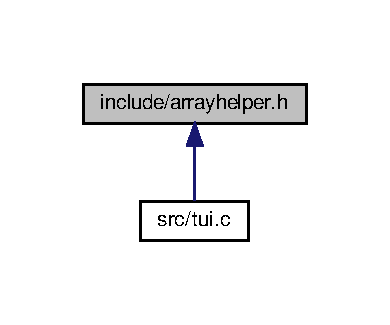
\includegraphics[width=187pt]{arrayhelper_8h__dep__incl}
\end{center}
\end{figure}
\subsection*{Macros}
\begin{DoxyCompactItemize}
\item 
\#define \hyperlink{arrayhelper_8h_a70c57aae3eb654e205459b4362c8089a}{A\+R\+R\+A\+Y\+\_\+\+S\+I\+ZE}(array)~(sizeof(array) / sizeof(array\mbox{[}0\mbox{]}))
\end{DoxyCompactItemize}


\subsection{Detailed Description}
A set of macros that help manage arrays. 

\begin{DoxyAuthor}{Author}
Zachary T. Hickman (zhickman) 
\end{DoxyAuthor}
\begin{DoxyRefDesc}{Bug}
\item[\hyperlink{bug__bug000001}{Bug}]No known bugs. \end{DoxyRefDesc}


\subsection{Macro Definition Documentation}
\mbox{\Hypertarget{arrayhelper_8h_a70c57aae3eb654e205459b4362c8089a}\label{arrayhelper_8h_a70c57aae3eb654e205459b4362c8089a}} 
\index{arrayhelper.\+h@{arrayhelper.\+h}!A\+R\+R\+A\+Y\+\_\+\+S\+I\+ZE@{A\+R\+R\+A\+Y\+\_\+\+S\+I\+ZE}}
\index{A\+R\+R\+A\+Y\+\_\+\+S\+I\+ZE@{A\+R\+R\+A\+Y\+\_\+\+S\+I\+ZE}!arrayhelper.\+h@{arrayhelper.\+h}}
\subsubsection{\texorpdfstring{A\+R\+R\+A\+Y\+\_\+\+S\+I\+ZE}{ARRAY\_SIZE}}
{\footnotesize\ttfamily \#define A\+R\+R\+A\+Y\+\_\+\+S\+I\+ZE(\begin{DoxyParamCaption}\item[{}]{array }\end{DoxyParamCaption})~(sizeof(array) / sizeof(array\mbox{[}0\mbox{]}))}


\hypertarget{charhelper_8h}{}\section{include/charhelper.h File Reference}
\label{charhelper_8h}\index{include/charhelper.\+h@{include/charhelper.\+h}}
This graph shows which files directly or indirectly include this file\+:\nopagebreak
\begin{figure}[H]
\begin{center}
\leavevmode
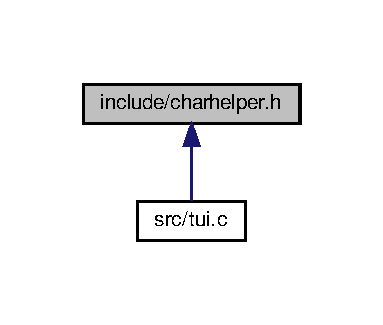
\includegraphics[width=184pt]{charhelper_8h__dep__incl}
\end{center}
\end{figure}
\subsection*{Macros}
\begin{DoxyCompactItemize}
\item 
\#define \hyperlink{charhelper_8h_ac763d1de8ee96951064bd7dbb649dfc5}{C\+H\+A\+R\+\_\+\+E\+SC}~\textquotesingle{}\textbackslash{}x1B\textquotesingle{}
\end{DoxyCompactItemize}


\subsection{Macro Definition Documentation}
\mbox{\Hypertarget{charhelper_8h_ac763d1de8ee96951064bd7dbb649dfc5}\label{charhelper_8h_ac763d1de8ee96951064bd7dbb649dfc5}} 
\index{charhelper.\+h@{charhelper.\+h}!C\+H\+A\+R\+\_\+\+E\+SC@{C\+H\+A\+R\+\_\+\+E\+SC}}
\index{C\+H\+A\+R\+\_\+\+E\+SC@{C\+H\+A\+R\+\_\+\+E\+SC}!charhelper.\+h@{charhelper.\+h}}
\subsubsection{\texorpdfstring{C\+H\+A\+R\+\_\+\+E\+SC}{CHAR\_ESC}}
{\footnotesize\ttfamily \#define C\+H\+A\+R\+\_\+\+E\+SC~\textquotesingle{}\textbackslash{}x1B\textquotesingle{}}


\hypertarget{mtxhelper_8h}{}\section{include/mtxhelper.h File Reference}
\label{mtxhelper_8h}\index{include/mtxhelper.\+h@{include/mtxhelper.\+h}}


A set of macros that help create, init, and control mutexes with variables.  


{\ttfamily \#include $<$pthread.\+h$>$}\newline
Include dependency graph for mtxhelper.\+h\+:\nopagebreak
\begin{figure}[H]
\begin{center}
\leavevmode
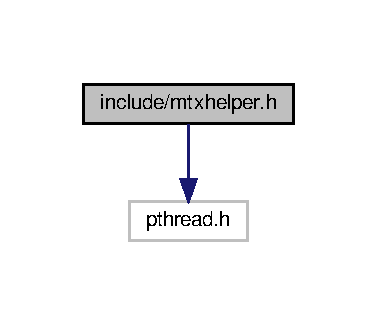
\includegraphics[width=181pt]{mtxhelper_8h__incl}
\end{center}
\end{figure}
This graph shows which files directly or indirectly include this file\+:\nopagebreak
\begin{figure}[H]
\begin{center}
\leavevmode
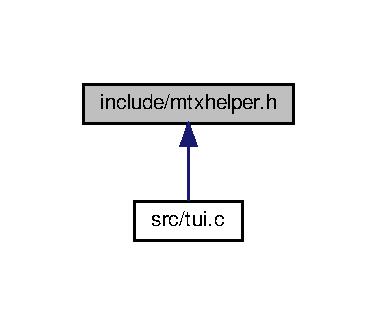
\includegraphics[width=181pt]{mtxhelper_8h__dep__incl}
\end{center}
\end{figure}
\subsection*{Macros}
\begin{DoxyCompactItemize}
\item 
\#define \hyperlink{mtxhelper_8h_af516bef484794c1e4ab0c3c344c3a2ba}{D\+E\+C\+L\+A\+R\+E\+\_\+\+M\+U\+T\+E\+X\+\_\+\+E\+X\+T\+E\+RN}(type,  name)~extern type name;
\item 
\#define \hyperlink{mtxhelper_8h_a0e72c8e164264aff1892337465db1698}{D\+E\+C\+L\+A\+R\+E\+\_\+\+M\+U\+T\+E\+X\+\_\+\+V\+AR}(type,  name)
\item 
\#define \hyperlink{mtxhelper_8h_a876dd8acada7f0e8102e6faeb82d1efa}{I\+N\+I\+T\+\_\+\+V\+A\+R\+\_\+\+M\+U\+T\+EX}(name)~pthread\+\_\+mutex\+\_\+init(\&name\+\_\+mutex, N\+U\+LL);
\item 
\#define \hyperlink{mtxhelper_8h_a55c0f67bdaea782c1da1e4642d6af0c2}{L\+O\+C\+K\+\_\+\+V\+A\+R\+\_\+\+M\+U\+T\+EX}(name)~pthread\+\_\+mutex\+\_\+lock(\&name\+\_\+mutex);
\item 
\#define \hyperlink{mtxhelper_8h_a32b4edda6cc315ec81e72099c7073258}{U\+N\+L\+O\+C\+K\+\_\+\+V\+A\+R\+\_\+\+M\+U\+T\+EX}(name)~pthread\+\_\+mutex\+\_\+unlock(\&name\+\_\+mutex);
\item 
\#define \hyperlink{mtxhelper_8h_a8d14cf3c28e9f1ed04025e7e34f584dc}{S\+E\+T\+\_\+\+M\+U\+T\+E\+X\+\_\+\+V\+AR}(name,  value)
\end{DoxyCompactItemize}


\subsection{Detailed Description}
A set of macros that help create, init, and control mutexes with variables. 

\begin{DoxyAuthor}{Author}
Zachary T. Hickman (zhickman) 
\end{DoxyAuthor}
\begin{DoxyRefDesc}{Bug}
\item[\hyperlink{bug__bug000002}{Bug}]No known bugs. \end{DoxyRefDesc}


\subsection{Macro Definition Documentation}
\mbox{\Hypertarget{mtxhelper_8h_af516bef484794c1e4ab0c3c344c3a2ba}\label{mtxhelper_8h_af516bef484794c1e4ab0c3c344c3a2ba}} 
\index{mtxhelper.\+h@{mtxhelper.\+h}!D\+E\+C\+L\+A\+R\+E\+\_\+\+M\+U\+T\+E\+X\+\_\+\+E\+X\+T\+E\+RN@{D\+E\+C\+L\+A\+R\+E\+\_\+\+M\+U\+T\+E\+X\+\_\+\+E\+X\+T\+E\+RN}}
\index{D\+E\+C\+L\+A\+R\+E\+\_\+\+M\+U\+T\+E\+X\+\_\+\+E\+X\+T\+E\+RN@{D\+E\+C\+L\+A\+R\+E\+\_\+\+M\+U\+T\+E\+X\+\_\+\+E\+X\+T\+E\+RN}!mtxhelper.\+h@{mtxhelper.\+h}}
\subsubsection{\texorpdfstring{D\+E\+C\+L\+A\+R\+E\+\_\+\+M\+U\+T\+E\+X\+\_\+\+E\+X\+T\+E\+RN}{DECLARE\_MUTEX\_EXTERN}}
{\footnotesize\ttfamily \#define D\+E\+C\+L\+A\+R\+E\+\_\+\+M\+U\+T\+E\+X\+\_\+\+E\+X\+T\+E\+RN(\begin{DoxyParamCaption}\item[{}]{type,  }\item[{}]{name }\end{DoxyParamCaption})~extern type name;}

\mbox{\Hypertarget{mtxhelper_8h_a0e72c8e164264aff1892337465db1698}\label{mtxhelper_8h_a0e72c8e164264aff1892337465db1698}} 
\index{mtxhelper.\+h@{mtxhelper.\+h}!D\+E\+C\+L\+A\+R\+E\+\_\+\+M\+U\+T\+E\+X\+\_\+\+V\+AR@{D\+E\+C\+L\+A\+R\+E\+\_\+\+M\+U\+T\+E\+X\+\_\+\+V\+AR}}
\index{D\+E\+C\+L\+A\+R\+E\+\_\+\+M\+U\+T\+E\+X\+\_\+\+V\+AR@{D\+E\+C\+L\+A\+R\+E\+\_\+\+M\+U\+T\+E\+X\+\_\+\+V\+AR}!mtxhelper.\+h@{mtxhelper.\+h}}
\subsubsection{\texorpdfstring{D\+E\+C\+L\+A\+R\+E\+\_\+\+M\+U\+T\+E\+X\+\_\+\+V\+AR}{DECLARE\_MUTEX\_VAR}}
{\footnotesize\ttfamily \#define D\+E\+C\+L\+A\+R\+E\+\_\+\+M\+U\+T\+E\+X\+\_\+\+V\+AR(\begin{DoxyParamCaption}\item[{}]{type,  }\item[{}]{name }\end{DoxyParamCaption})}

{\bfseries Value\+:}
\begin{DoxyCode}
\textcolor{keyword}{volatile} type name; \(\backslash\)
    pthread\_mutex\_t name\_mutex;
\end{DoxyCode}
\mbox{\Hypertarget{mtxhelper_8h_a876dd8acada7f0e8102e6faeb82d1efa}\label{mtxhelper_8h_a876dd8acada7f0e8102e6faeb82d1efa}} 
\index{mtxhelper.\+h@{mtxhelper.\+h}!I\+N\+I\+T\+\_\+\+V\+A\+R\+\_\+\+M\+U\+T\+EX@{I\+N\+I\+T\+\_\+\+V\+A\+R\+\_\+\+M\+U\+T\+EX}}
\index{I\+N\+I\+T\+\_\+\+V\+A\+R\+\_\+\+M\+U\+T\+EX@{I\+N\+I\+T\+\_\+\+V\+A\+R\+\_\+\+M\+U\+T\+EX}!mtxhelper.\+h@{mtxhelper.\+h}}
\subsubsection{\texorpdfstring{I\+N\+I\+T\+\_\+\+V\+A\+R\+\_\+\+M\+U\+T\+EX}{INIT\_VAR\_MUTEX}}
{\footnotesize\ttfamily \#define I\+N\+I\+T\+\_\+\+V\+A\+R\+\_\+\+M\+U\+T\+EX(\begin{DoxyParamCaption}\item[{}]{name }\end{DoxyParamCaption})~pthread\+\_\+mutex\+\_\+init(\&name\+\_\+mutex, N\+U\+LL);}

\mbox{\Hypertarget{mtxhelper_8h_a55c0f67bdaea782c1da1e4642d6af0c2}\label{mtxhelper_8h_a55c0f67bdaea782c1da1e4642d6af0c2}} 
\index{mtxhelper.\+h@{mtxhelper.\+h}!L\+O\+C\+K\+\_\+\+V\+A\+R\+\_\+\+M\+U\+T\+EX@{L\+O\+C\+K\+\_\+\+V\+A\+R\+\_\+\+M\+U\+T\+EX}}
\index{L\+O\+C\+K\+\_\+\+V\+A\+R\+\_\+\+M\+U\+T\+EX@{L\+O\+C\+K\+\_\+\+V\+A\+R\+\_\+\+M\+U\+T\+EX}!mtxhelper.\+h@{mtxhelper.\+h}}
\subsubsection{\texorpdfstring{L\+O\+C\+K\+\_\+\+V\+A\+R\+\_\+\+M\+U\+T\+EX}{LOCK\_VAR\_MUTEX}}
{\footnotesize\ttfamily \#define L\+O\+C\+K\+\_\+\+V\+A\+R\+\_\+\+M\+U\+T\+EX(\begin{DoxyParamCaption}\item[{}]{name }\end{DoxyParamCaption})~pthread\+\_\+mutex\+\_\+lock(\&name\+\_\+mutex);}

\mbox{\Hypertarget{mtxhelper_8h_a8d14cf3c28e9f1ed04025e7e34f584dc}\label{mtxhelper_8h_a8d14cf3c28e9f1ed04025e7e34f584dc}} 
\index{mtxhelper.\+h@{mtxhelper.\+h}!S\+E\+T\+\_\+\+M\+U\+T\+E\+X\+\_\+\+V\+AR@{S\+E\+T\+\_\+\+M\+U\+T\+E\+X\+\_\+\+V\+AR}}
\index{S\+E\+T\+\_\+\+M\+U\+T\+E\+X\+\_\+\+V\+AR@{S\+E\+T\+\_\+\+M\+U\+T\+E\+X\+\_\+\+V\+AR}!mtxhelper.\+h@{mtxhelper.\+h}}
\subsubsection{\texorpdfstring{S\+E\+T\+\_\+\+M\+U\+T\+E\+X\+\_\+\+V\+AR}{SET\_MUTEX\_VAR}}
{\footnotesize\ttfamily \#define S\+E\+T\+\_\+\+M\+U\+T\+E\+X\+\_\+\+V\+AR(\begin{DoxyParamCaption}\item[{}]{name,  }\item[{}]{value }\end{DoxyParamCaption})}

{\bfseries Value\+:}
\begin{DoxyCode}
\hyperlink{mtxhelper_8h_a55c0f67bdaea782c1da1e4642d6af0c2}{LOCK\_VAR\_MUTEX}(name) \(\backslash\)
    name = value; \(\backslash\)
    UNLOCK\_VAR\_MUTEX(name)
\end{DoxyCode}
\mbox{\Hypertarget{mtxhelper_8h_a32b4edda6cc315ec81e72099c7073258}\label{mtxhelper_8h_a32b4edda6cc315ec81e72099c7073258}} 
\index{mtxhelper.\+h@{mtxhelper.\+h}!U\+N\+L\+O\+C\+K\+\_\+\+V\+A\+R\+\_\+\+M\+U\+T\+EX@{U\+N\+L\+O\+C\+K\+\_\+\+V\+A\+R\+\_\+\+M\+U\+T\+EX}}
\index{U\+N\+L\+O\+C\+K\+\_\+\+V\+A\+R\+\_\+\+M\+U\+T\+EX@{U\+N\+L\+O\+C\+K\+\_\+\+V\+A\+R\+\_\+\+M\+U\+T\+EX}!mtxhelper.\+h@{mtxhelper.\+h}}
\subsubsection{\texorpdfstring{U\+N\+L\+O\+C\+K\+\_\+\+V\+A\+R\+\_\+\+M\+U\+T\+EX}{UNLOCK\_VAR\_MUTEX}}
{\footnotesize\ttfamily \#define U\+N\+L\+O\+C\+K\+\_\+\+V\+A\+R\+\_\+\+M\+U\+T\+EX(\begin{DoxyParamCaption}\item[{}]{name }\end{DoxyParamCaption})~pthread\+\_\+mutex\+\_\+unlock(\&name\+\_\+mutex);}


\hypertarget{tui_8h}{}\section{include/tui.h File Reference}
\label{tui_8h}\index{include/tui.\+h@{include/tui.\+h}}
This graph shows which files directly or indirectly include this file\+:\nopagebreak
\begin{figure}[H]
\begin{center}
\leavevmode
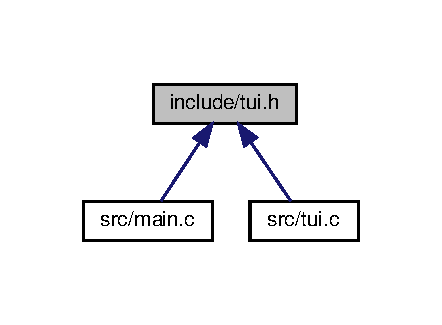
\includegraphics[width=212pt]{tui_8h__dep__incl}
\end{center}
\end{figure}
\subsection*{Macros}
\begin{DoxyCompactItemize}
\item 
\#define \hyperlink{tui_8h_a3e14de130f00b1dbd4ca02ddf5623e71}{C\+O\+L\+O\+R\+P\+A\+I\+R\+\_\+\+W\+H\+I\+T\+E\+\_\+\+B\+L\+A\+CK}~1
\begin{DoxyCompactList}\small\item\em Define color pair indexes to use with ncurses. \end{DoxyCompactList}\item 
\#define \hyperlink{tui_8h_ad13525c8d019e074e260b53dd183f4a4}{C\+O\+L\+O\+R\+P\+A\+I\+R\+\_\+\+B\+L\+A\+C\+K\+\_\+\+W\+H\+I\+TE}~2
\item 
\#define \hyperlink{tui_8h_aa3e669c9eb82b0cad4f4559695138b45}{C\+O\+L\+O\+R\+P\+A\+I\+R\+\_\+\+W\+H\+I\+T\+E\+\_\+\+B\+L\+UE}~3
\item 
\#define \hyperlink{tui_8h_a418937537dbeb18fb35c7b7d6f743c20}{C\+O\+L\+O\+R\+P\+A\+I\+R\+\_\+\+B\+L\+U\+E\+\_\+\+W\+H\+I\+TE}~4
\end{DoxyCompactItemize}
\subsection*{Functions}
\begin{DoxyCompactItemize}
\item 
int \hyperlink{tui_8h_a50220f3c4859104f84b4b5b06f6074fe}{tui\+\_\+handle\+\_\+input} ()
\item 
void \hyperlink{tui_8h_a933a448d1adf3cac78fd3a75f729a521}{tui\+\_\+resize\+\_\+handler} (int sig)
\item 
void \hyperlink{tui_8h_a273e0f27732fe6b4c2644927a14e9428}{tui\+\_\+init} ()
\begin{DoxyCompactList}\small\item\em H\+I\+FN Initializes the UI interface, and panels. \end{DoxyCompactList}\item 
void \hyperlink{tui_8h_aad57a653d5bc57141d3bb73b4a29b9e9}{tui\+\_\+stop} ()
\begin{DoxyCompactList}\small\item\em H\+I\+FN Deinitializes the UI interface and panels. \end{DoxyCompactList}\item 
void \hyperlink{tui_8h_a37ebe23d01d303deb649c64afb7b68ea}{tui\+\_\+update\+\_\+ui} ()
\end{DoxyCompactItemize}


\subsection{Macro Definition Documentation}
\mbox{\Hypertarget{tui_8h_ad13525c8d019e074e260b53dd183f4a4}\label{tui_8h_ad13525c8d019e074e260b53dd183f4a4}} 
\index{tui.\+h@{tui.\+h}!C\+O\+L\+O\+R\+P\+A\+I\+R\+\_\+\+B\+L\+A\+C\+K\+\_\+\+W\+H\+I\+TE@{C\+O\+L\+O\+R\+P\+A\+I\+R\+\_\+\+B\+L\+A\+C\+K\+\_\+\+W\+H\+I\+TE}}
\index{C\+O\+L\+O\+R\+P\+A\+I\+R\+\_\+\+B\+L\+A\+C\+K\+\_\+\+W\+H\+I\+TE@{C\+O\+L\+O\+R\+P\+A\+I\+R\+\_\+\+B\+L\+A\+C\+K\+\_\+\+W\+H\+I\+TE}!tui.\+h@{tui.\+h}}
\subsubsection{\texorpdfstring{C\+O\+L\+O\+R\+P\+A\+I\+R\+\_\+\+B\+L\+A\+C\+K\+\_\+\+W\+H\+I\+TE}{COLORPAIR\_BLACK\_WHITE}}
{\footnotesize\ttfamily \#define C\+O\+L\+O\+R\+P\+A\+I\+R\+\_\+\+B\+L\+A\+C\+K\+\_\+\+W\+H\+I\+TE~2}

\mbox{\Hypertarget{tui_8h_a418937537dbeb18fb35c7b7d6f743c20}\label{tui_8h_a418937537dbeb18fb35c7b7d6f743c20}} 
\index{tui.\+h@{tui.\+h}!C\+O\+L\+O\+R\+P\+A\+I\+R\+\_\+\+B\+L\+U\+E\+\_\+\+W\+H\+I\+TE@{C\+O\+L\+O\+R\+P\+A\+I\+R\+\_\+\+B\+L\+U\+E\+\_\+\+W\+H\+I\+TE}}
\index{C\+O\+L\+O\+R\+P\+A\+I\+R\+\_\+\+B\+L\+U\+E\+\_\+\+W\+H\+I\+TE@{C\+O\+L\+O\+R\+P\+A\+I\+R\+\_\+\+B\+L\+U\+E\+\_\+\+W\+H\+I\+TE}!tui.\+h@{tui.\+h}}
\subsubsection{\texorpdfstring{C\+O\+L\+O\+R\+P\+A\+I\+R\+\_\+\+B\+L\+U\+E\+\_\+\+W\+H\+I\+TE}{COLORPAIR\_BLUE\_WHITE}}
{\footnotesize\ttfamily \#define C\+O\+L\+O\+R\+P\+A\+I\+R\+\_\+\+B\+L\+U\+E\+\_\+\+W\+H\+I\+TE~4}

\mbox{\Hypertarget{tui_8h_a3e14de130f00b1dbd4ca02ddf5623e71}\label{tui_8h_a3e14de130f00b1dbd4ca02ddf5623e71}} 
\index{tui.\+h@{tui.\+h}!C\+O\+L\+O\+R\+P\+A\+I\+R\+\_\+\+W\+H\+I\+T\+E\+\_\+\+B\+L\+A\+CK@{C\+O\+L\+O\+R\+P\+A\+I\+R\+\_\+\+W\+H\+I\+T\+E\+\_\+\+B\+L\+A\+CK}}
\index{C\+O\+L\+O\+R\+P\+A\+I\+R\+\_\+\+W\+H\+I\+T\+E\+\_\+\+B\+L\+A\+CK@{C\+O\+L\+O\+R\+P\+A\+I\+R\+\_\+\+W\+H\+I\+T\+E\+\_\+\+B\+L\+A\+CK}!tui.\+h@{tui.\+h}}
\subsubsection{\texorpdfstring{C\+O\+L\+O\+R\+P\+A\+I\+R\+\_\+\+W\+H\+I\+T\+E\+\_\+\+B\+L\+A\+CK}{COLORPAIR\_WHITE\_BLACK}}
{\footnotesize\ttfamily \#define C\+O\+L\+O\+R\+P\+A\+I\+R\+\_\+\+W\+H\+I\+T\+E\+\_\+\+B\+L\+A\+CK~1}



Define color pair indexes to use with ncurses. 

\mbox{\Hypertarget{tui_8h_aa3e669c9eb82b0cad4f4559695138b45}\label{tui_8h_aa3e669c9eb82b0cad4f4559695138b45}} 
\index{tui.\+h@{tui.\+h}!C\+O\+L\+O\+R\+P\+A\+I\+R\+\_\+\+W\+H\+I\+T\+E\+\_\+\+B\+L\+UE@{C\+O\+L\+O\+R\+P\+A\+I\+R\+\_\+\+W\+H\+I\+T\+E\+\_\+\+B\+L\+UE}}
\index{C\+O\+L\+O\+R\+P\+A\+I\+R\+\_\+\+W\+H\+I\+T\+E\+\_\+\+B\+L\+UE@{C\+O\+L\+O\+R\+P\+A\+I\+R\+\_\+\+W\+H\+I\+T\+E\+\_\+\+B\+L\+UE}!tui.\+h@{tui.\+h}}
\subsubsection{\texorpdfstring{C\+O\+L\+O\+R\+P\+A\+I\+R\+\_\+\+W\+H\+I\+T\+E\+\_\+\+B\+L\+UE}{COLORPAIR\_WHITE\_BLUE}}
{\footnotesize\ttfamily \#define C\+O\+L\+O\+R\+P\+A\+I\+R\+\_\+\+W\+H\+I\+T\+E\+\_\+\+B\+L\+UE~3}



\subsection{Function Documentation}
\mbox{\Hypertarget{tui_8h_a50220f3c4859104f84b4b5b06f6074fe}\label{tui_8h_a50220f3c4859104f84b4b5b06f6074fe}} 
\index{tui.\+h@{tui.\+h}!tui\+\_\+handle\+\_\+input@{tui\+\_\+handle\+\_\+input}}
\index{tui\+\_\+handle\+\_\+input@{tui\+\_\+handle\+\_\+input}!tui.\+h@{tui.\+h}}
\subsubsection{\texorpdfstring{tui\+\_\+handle\+\_\+input()}{tui\_handle\_input()}}
{\footnotesize\ttfamily int tui\+\_\+handle\+\_\+input (\begin{DoxyParamCaption}{ }\end{DoxyParamCaption})}

Here is the caller graph for this function\+:\nopagebreak
\begin{figure}[H]
\begin{center}
\leavevmode
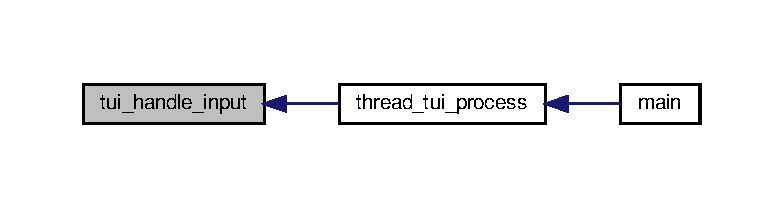
\includegraphics[width=350pt]{tui_8h_a50220f3c4859104f84b4b5b06f6074fe_icgraph}
\end{center}
\end{figure}
\mbox{\Hypertarget{tui_8h_a273e0f27732fe6b4c2644927a14e9428}\label{tui_8h_a273e0f27732fe6b4c2644927a14e9428}} 
\index{tui.\+h@{tui.\+h}!tui\+\_\+init@{tui\+\_\+init}}
\index{tui\+\_\+init@{tui\+\_\+init}!tui.\+h@{tui.\+h}}
\subsubsection{\texorpdfstring{tui\+\_\+init()}{tui\_init()}}
{\footnotesize\ttfamily void tui\+\_\+init (\begin{DoxyParamCaption}{ }\end{DoxyParamCaption})}



H\+I\+FN Initializes the UI interface, and panels. 

Here is the call graph for this function\+:\nopagebreak
\begin{figure}[H]
\begin{center}
\leavevmode
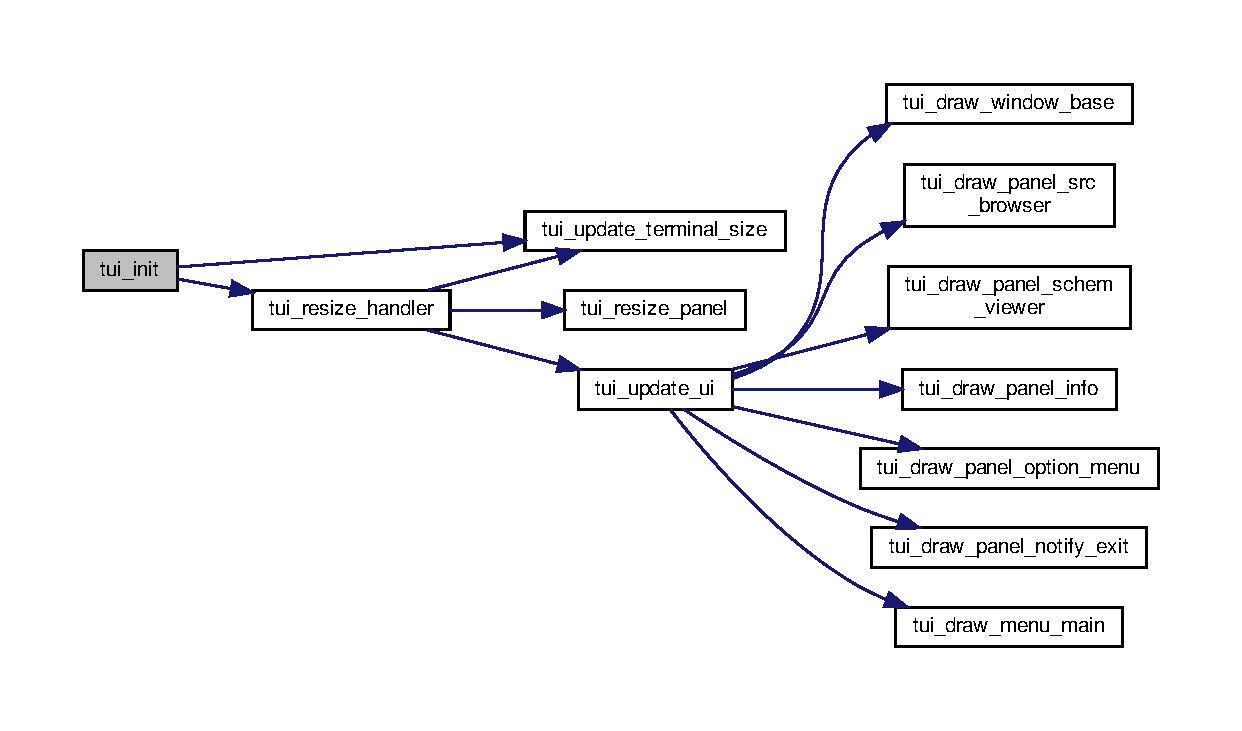
\includegraphics[width=350pt]{tui_8h_a273e0f27732fe6b4c2644927a14e9428_cgraph}
\end{center}
\end{figure}
Here is the caller graph for this function\+:\nopagebreak
\begin{figure}[H]
\begin{center}
\leavevmode
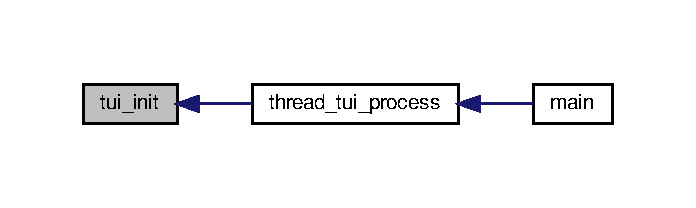
\includegraphics[width=334pt]{tui_8h_a273e0f27732fe6b4c2644927a14e9428_icgraph}
\end{center}
\end{figure}
\mbox{\Hypertarget{tui_8h_a933a448d1adf3cac78fd3a75f729a521}\label{tui_8h_a933a448d1adf3cac78fd3a75f729a521}} 
\index{tui.\+h@{tui.\+h}!tui\+\_\+resize\+\_\+handler@{tui\+\_\+resize\+\_\+handler}}
\index{tui\+\_\+resize\+\_\+handler@{tui\+\_\+resize\+\_\+handler}!tui.\+h@{tui.\+h}}
\subsubsection{\texorpdfstring{tui\+\_\+resize\+\_\+handler()}{tui\_resize\_handler()}}
{\footnotesize\ttfamily void tui\+\_\+resize\+\_\+handler (\begin{DoxyParamCaption}\item[{int}]{sig }\end{DoxyParamCaption})}

Here is the call graph for this function\+:\nopagebreak
\begin{figure}[H]
\begin{center}
\leavevmode
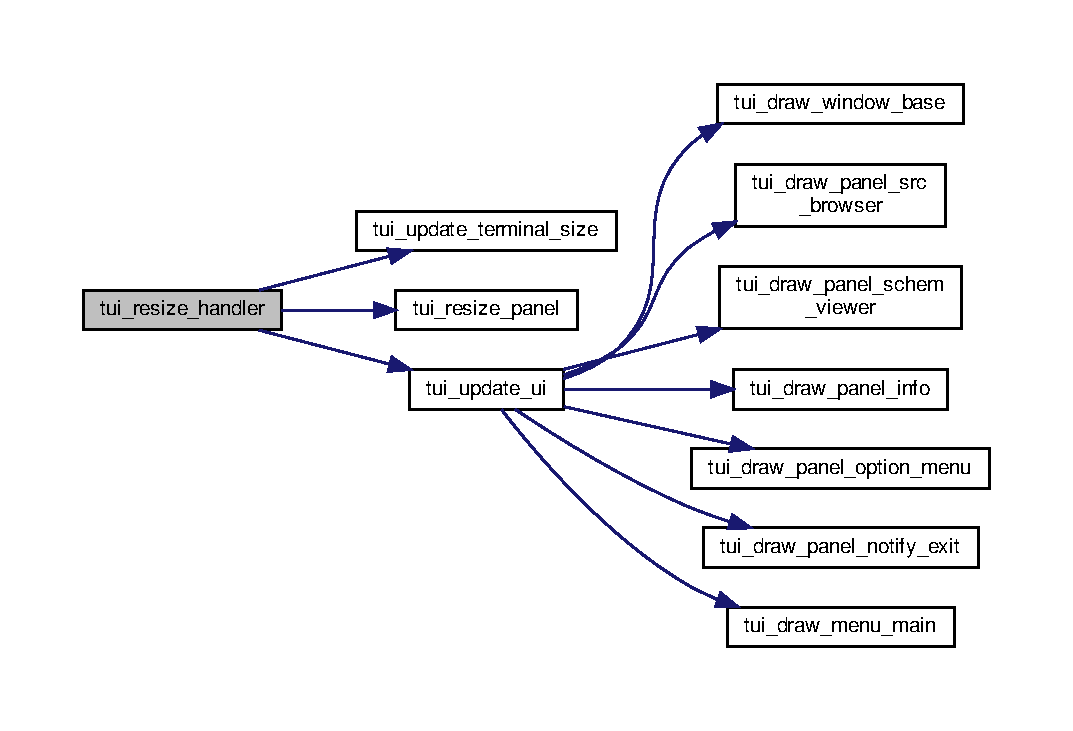
\includegraphics[width=350pt]{tui_8h_a933a448d1adf3cac78fd3a75f729a521_cgraph}
\end{center}
\end{figure}
Here is the caller graph for this function\+:\nopagebreak
\begin{figure}[H]
\begin{center}
\leavevmode
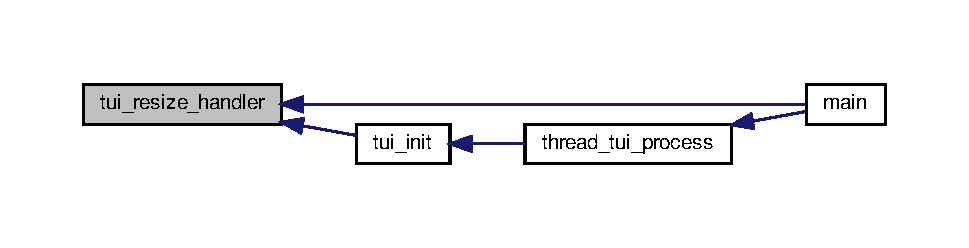
\includegraphics[width=350pt]{tui_8h_a933a448d1adf3cac78fd3a75f729a521_icgraph}
\end{center}
\end{figure}
\mbox{\Hypertarget{tui_8h_aad57a653d5bc57141d3bb73b4a29b9e9}\label{tui_8h_aad57a653d5bc57141d3bb73b4a29b9e9}} 
\index{tui.\+h@{tui.\+h}!tui\+\_\+stop@{tui\+\_\+stop}}
\index{tui\+\_\+stop@{tui\+\_\+stop}!tui.\+h@{tui.\+h}}
\subsubsection{\texorpdfstring{tui\+\_\+stop()}{tui\_stop()}}
{\footnotesize\ttfamily void tui\+\_\+stop (\begin{DoxyParamCaption}{ }\end{DoxyParamCaption})}



H\+I\+FN Deinitializes the UI interface and panels. 

Here is the caller graph for this function\+:\nopagebreak
\begin{figure}[H]
\begin{center}
\leavevmode
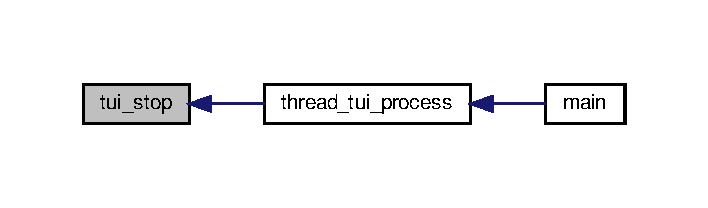
\includegraphics[width=340pt]{tui_8h_aad57a653d5bc57141d3bb73b4a29b9e9_icgraph}
\end{center}
\end{figure}
\mbox{\Hypertarget{tui_8h_a37ebe23d01d303deb649c64afb7b68ea}\label{tui_8h_a37ebe23d01d303deb649c64afb7b68ea}} 
\index{tui.\+h@{tui.\+h}!tui\+\_\+update\+\_\+ui@{tui\+\_\+update\+\_\+ui}}
\index{tui\+\_\+update\+\_\+ui@{tui\+\_\+update\+\_\+ui}!tui.\+h@{tui.\+h}}
\subsubsection{\texorpdfstring{tui\+\_\+update\+\_\+ui()}{tui\_update\_ui()}}
{\footnotesize\ttfamily void tui\+\_\+update\+\_\+ui (\begin{DoxyParamCaption}{ }\end{DoxyParamCaption})}

Here is the call graph for this function\+:\nopagebreak
\begin{figure}[H]
\begin{center}
\leavevmode
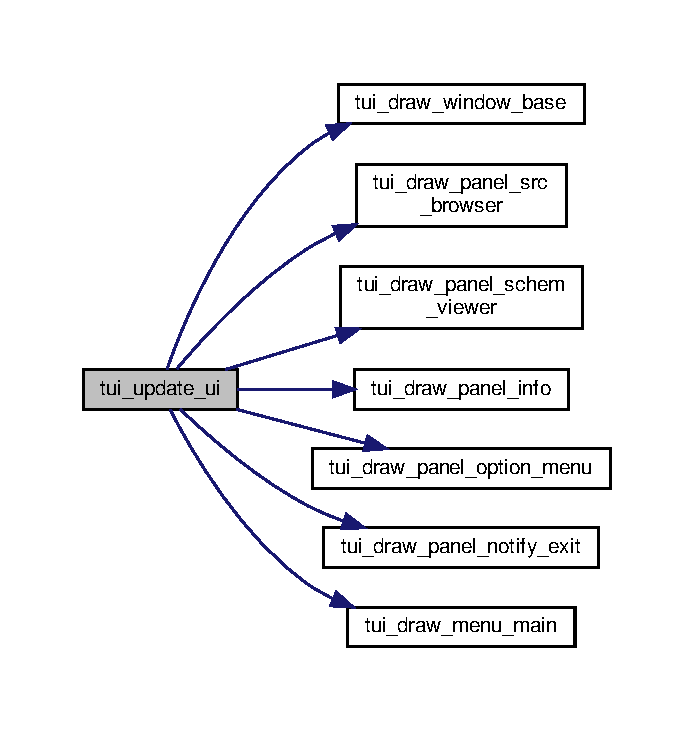
\includegraphics[width=333pt]{tui_8h_a37ebe23d01d303deb649c64afb7b68ea_cgraph}
\end{center}
\end{figure}
Here is the caller graph for this function\+:\nopagebreak
\begin{figure}[H]
\begin{center}
\leavevmode
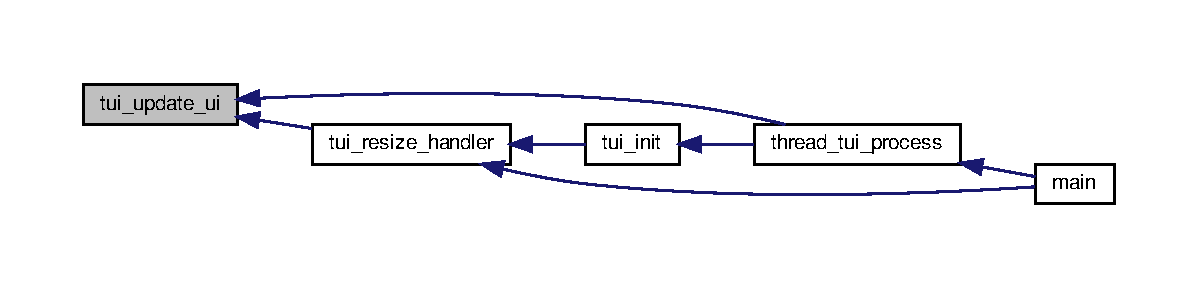
\includegraphics[width=350pt]{tui_8h_a37ebe23d01d303deb649c64afb7b68ea_icgraph}
\end{center}
\end{figure}

\hypertarget{main_8c}{}\section{src/main.c File Reference}
\label{main_8c}\index{src/main.\+c@{src/main.\+c}}
{\ttfamily \#include $<$stdlib.\+h$>$}\newline
{\ttfamily \#include $<$stdbool.\+h$>$}\newline
{\ttfamily \#include $<$stdio.\+h$>$}\newline
{\ttfamily \#include $<$unistd.\+h$>$}\newline
{\ttfamily \#include $<$signal.\+h$>$}\newline
{\ttfamily \#include $<$pthread.\+h$>$}\newline
{\ttfamily \#include $<$readline/readline.\+h$>$}\newline
{\ttfamily \#include \char`\"{}tui.\+h\char`\"{}}\newline
Include dependency graph for main.\+c\+:\nopagebreak
\begin{figure}[H]
\begin{center}
\leavevmode
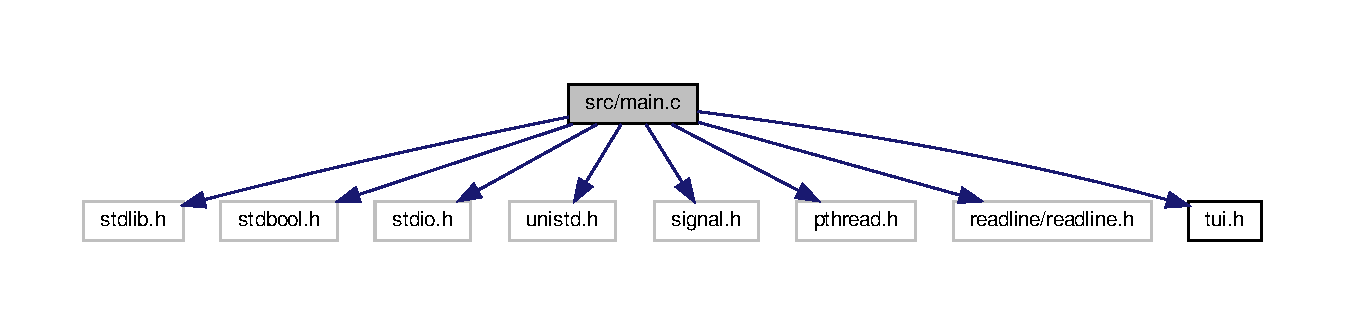
\includegraphics[width=350pt]{main_8c__incl}
\end{center}
\end{figure}
\subsection*{Functions}
\begin{DoxyCompactItemize}
\item 
void \hyperlink{main_8c_a1a87b5de5ced9dbf84b4feefc3b01ccf}{main\+\_\+int\+\_\+handler} (int signum)
\begin{DoxyCompactList}\small\item\em Catches S\+I\+G\+I\+NT, and flags an exit is requested. \end{DoxyCompactList}\item 
void $\ast$ \hyperlink{main_8c_a20debbe95676c5ff3a1a27dbfa796ae9}{thread\+\_\+tui\+\_\+process} (void $\ast$vargp)
\begin{DoxyCompactList}\small\item\em Threaded function for T\+UI. \end{DoxyCompactList}\item 
int \hyperlink{main_8c_a0ddf1224851353fc92bfbff6f499fa97}{main} (int argc, char $\ast$argv\mbox{[}$\,$\mbox{]})
\end{DoxyCompactItemize}
\subsection*{Variables}
\begin{DoxyCompactItemize}
\item 
pthread\+\_\+t \hyperlink{main_8c_ae5bdba207b41f4c04ed1fa44c551d2a4}{tid\+\_\+tui}
\begin{DoxyCompactList}\small\item\em Declare T\+UI thread id storage. \end{DoxyCompactList}\item 
volatile bool \hyperlink{main_8c_acfdf41beb20339e3a44000934094a8df}{caught\+\_\+sigint} = false
\begin{DoxyCompactList}\small\item\em Declare bool for if we caught a signit. \end{DoxyCompactList}\item 
volatile bool \hyperlink{main_8c_a73a1fdd4265d86440f3a2a444db31e0b}{do\+\_\+exit} = false
\end{DoxyCompactItemize}


\subsection{Function Documentation}
\mbox{\Hypertarget{main_8c_a0ddf1224851353fc92bfbff6f499fa97}\label{main_8c_a0ddf1224851353fc92bfbff6f499fa97}} 
\index{main.\+c@{main.\+c}!main@{main}}
\index{main@{main}!main.\+c@{main.\+c}}
\subsubsection{\texorpdfstring{main()}{main()}}
{\footnotesize\ttfamily int main (\begin{DoxyParamCaption}\item[{int}]{argc,  }\item[{char $\ast$}]{argv\mbox{[}$\,$\mbox{]} }\end{DoxyParamCaption})}

Here is the call graph for this function\+:\nopagebreak
\begin{figure}[H]
\begin{center}
\leavevmode
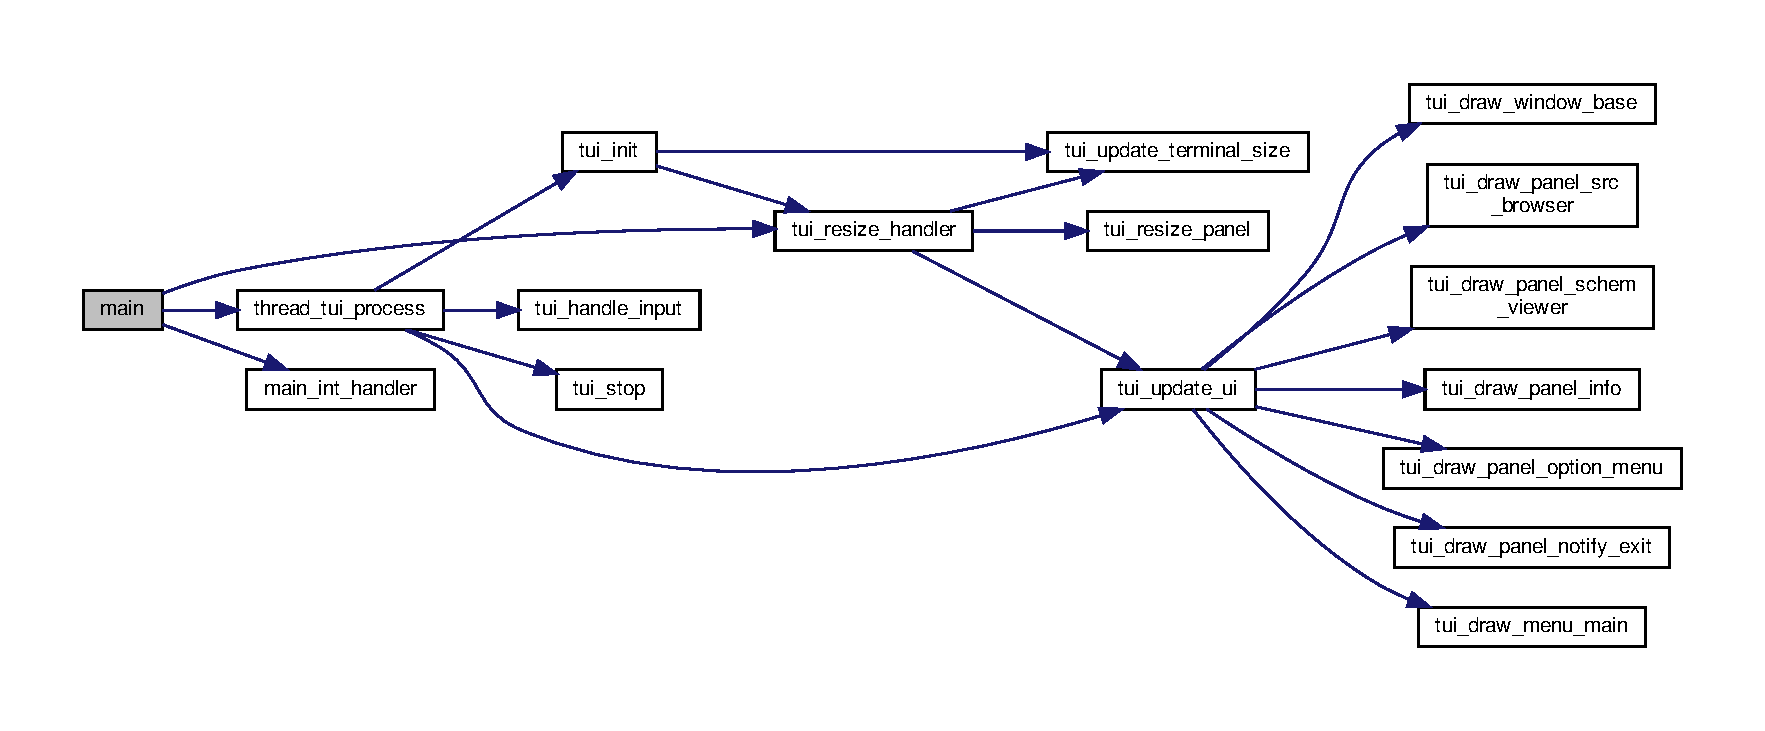
\includegraphics[width=350pt]{main_8c_a0ddf1224851353fc92bfbff6f499fa97_cgraph}
\end{center}
\end{figure}
\mbox{\Hypertarget{main_8c_a1a87b5de5ced9dbf84b4feefc3b01ccf}\label{main_8c_a1a87b5de5ced9dbf84b4feefc3b01ccf}} 
\index{main.\+c@{main.\+c}!main\+\_\+int\+\_\+handler@{main\+\_\+int\+\_\+handler}}
\index{main\+\_\+int\+\_\+handler@{main\+\_\+int\+\_\+handler}!main.\+c@{main.\+c}}
\subsubsection{\texorpdfstring{main\+\_\+int\+\_\+handler()}{main\_int\_handler()}}
{\footnotesize\ttfamily void main\+\_\+int\+\_\+handler (\begin{DoxyParamCaption}\item[{int}]{signum }\end{DoxyParamCaption})}



Catches S\+I\+G\+I\+NT, and flags an exit is requested. 

Here is the caller graph for this function\+:\nopagebreak
\begin{figure}[H]
\begin{center}
\leavevmode
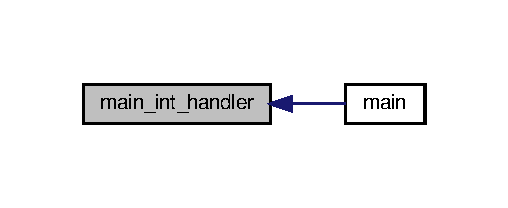
\includegraphics[width=244pt]{main_8c_a1a87b5de5ced9dbf84b4feefc3b01ccf_icgraph}
\end{center}
\end{figure}
\mbox{\Hypertarget{main_8c_a20debbe95676c5ff3a1a27dbfa796ae9}\label{main_8c_a20debbe95676c5ff3a1a27dbfa796ae9}} 
\index{main.\+c@{main.\+c}!thread\+\_\+tui\+\_\+process@{thread\+\_\+tui\+\_\+process}}
\index{thread\+\_\+tui\+\_\+process@{thread\+\_\+tui\+\_\+process}!main.\+c@{main.\+c}}
\subsubsection{\texorpdfstring{thread\+\_\+tui\+\_\+process()}{thread\_tui\_process()}}
{\footnotesize\ttfamily void$\ast$ thread\+\_\+tui\+\_\+process (\begin{DoxyParamCaption}\item[{void $\ast$}]{vargp }\end{DoxyParamCaption})}



Threaded function for T\+UI. 

Here is the call graph for this function\+:\nopagebreak
\begin{figure}[H]
\begin{center}
\leavevmode
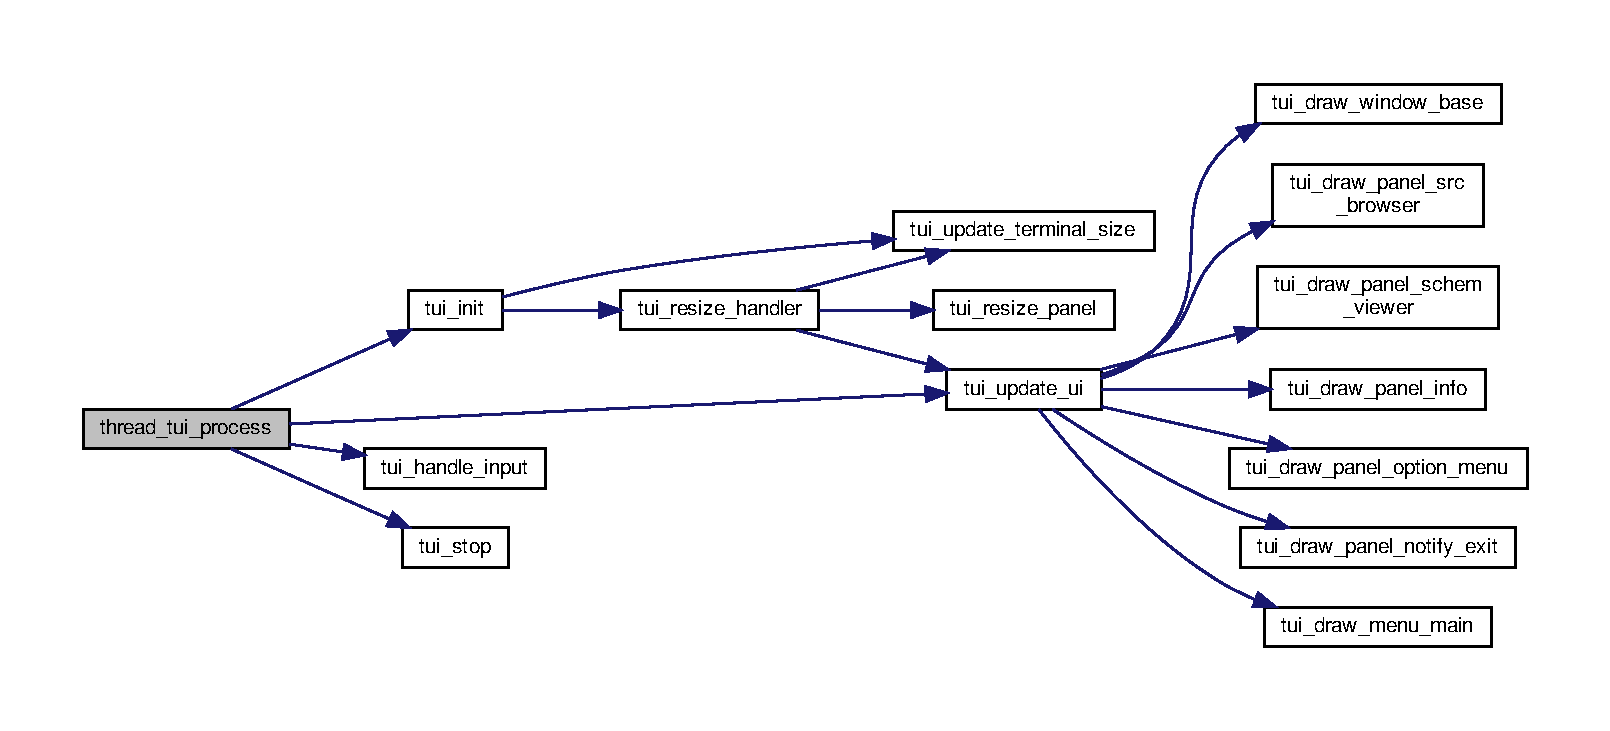
\includegraphics[width=350pt]{main_8c_a20debbe95676c5ff3a1a27dbfa796ae9_cgraph}
\end{center}
\end{figure}
Here is the caller graph for this function\+:\nopagebreak
\begin{figure}[H]
\begin{center}
\leavevmode
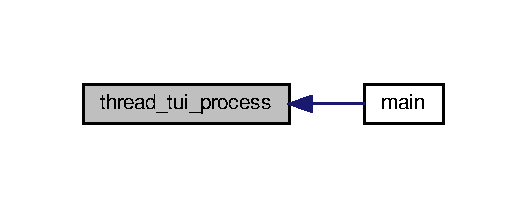
\includegraphics[width=253pt]{main_8c_a20debbe95676c5ff3a1a27dbfa796ae9_icgraph}
\end{center}
\end{figure}


\subsection{Variable Documentation}
\mbox{\Hypertarget{main_8c_acfdf41beb20339e3a44000934094a8df}\label{main_8c_acfdf41beb20339e3a44000934094a8df}} 
\index{main.\+c@{main.\+c}!caught\+\_\+sigint@{caught\+\_\+sigint}}
\index{caught\+\_\+sigint@{caught\+\_\+sigint}!main.\+c@{main.\+c}}
\subsubsection{\texorpdfstring{caught\+\_\+sigint}{caught\_sigint}}
{\footnotesize\ttfamily volatile bool caught\+\_\+sigint = false}



Declare bool for if we caught a signit. 

\mbox{\Hypertarget{main_8c_a73a1fdd4265d86440f3a2a444db31e0b}\label{main_8c_a73a1fdd4265d86440f3a2a444db31e0b}} 
\index{main.\+c@{main.\+c}!do\+\_\+exit@{do\+\_\+exit}}
\index{do\+\_\+exit@{do\+\_\+exit}!main.\+c@{main.\+c}}
\subsubsection{\texorpdfstring{do\+\_\+exit}{do\_exit}}
{\footnotesize\ttfamily volatile bool do\+\_\+exit = false}

\mbox{\Hypertarget{main_8c_ae5bdba207b41f4c04ed1fa44c551d2a4}\label{main_8c_ae5bdba207b41f4c04ed1fa44c551d2a4}} 
\index{main.\+c@{main.\+c}!tid\+\_\+tui@{tid\+\_\+tui}}
\index{tid\+\_\+tui@{tid\+\_\+tui}!main.\+c@{main.\+c}}
\subsubsection{\texorpdfstring{tid\+\_\+tui}{tid\_tui}}
{\footnotesize\ttfamily pthread\+\_\+t tid\+\_\+tui}



Declare T\+UI thread id storage. 


\hypertarget{tui_8c}{}\section{src/tui.c File Reference}
\label{tui_8c}\index{src/tui.\+c@{src/tui.\+c}}
{\ttfamily \#include $<$stdlib.\+h$>$}\newline
{\ttfamily \#include $<$signal.\+h$>$}\newline
{\ttfamily \#include $<$pthread.\+h$>$}\newline
{\ttfamily \#include $<$string.\+h$>$}\newline
{\ttfamily \#include $<$ncurses.\+h$>$}\newline
{\ttfamily \#include $<$panel.\+h$>$}\newline
{\ttfamily \#include $<$locale.\+h$>$}\newline
{\ttfamily \#include \char`\"{}mtxhelper.\+h\char`\"{}}\newline
{\ttfamily \#include \char`\"{}arrayhelper.\+h\char`\"{}}\newline
{\ttfamily \#include \char`\"{}charhelper.\+h\char`\"{}}\newline
{\ttfamily \#include \char`\"{}tui.\+h\char`\"{}}\newline
Include dependency graph for tui.\+c\+:\nopagebreak
\begin{figure}[H]
\begin{center}
\leavevmode
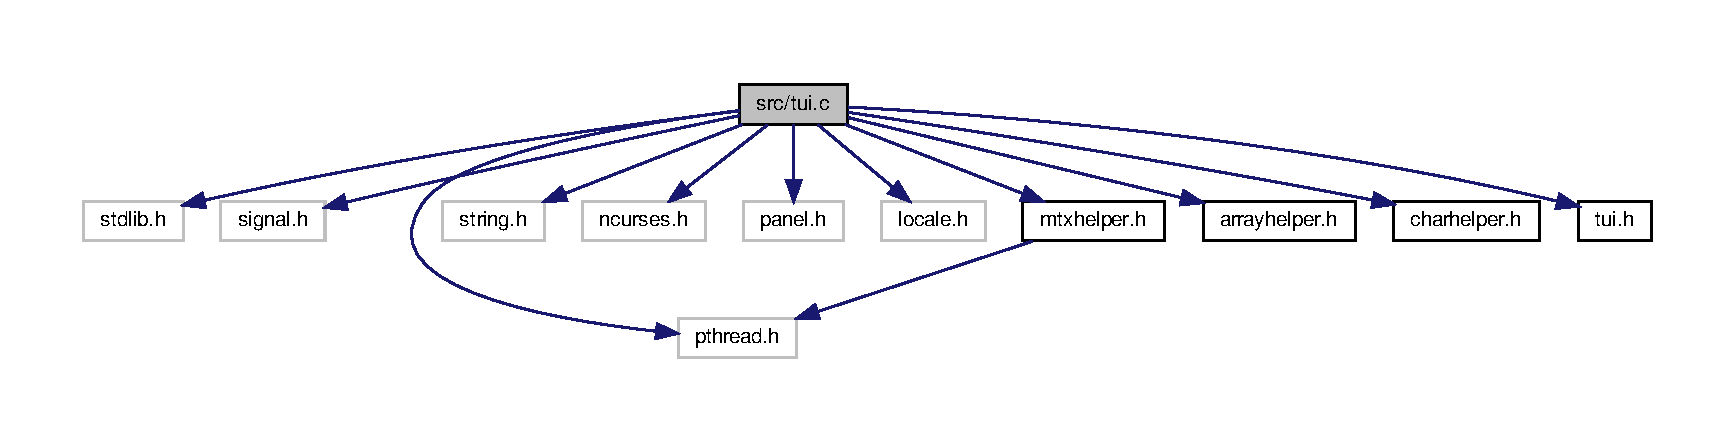
\includegraphics[width=350pt]{tui_8c__incl}
\end{center}
\end{figure}
\subsection*{Functions}
\begin{DoxyCompactItemize}
\item 
void \hyperlink{tui_8c_a1950cd06f7947f91941838bf3ed64f7f}{tui\+\_\+draw\+\_\+window\+\_\+base} ()
\item 
void \hyperlink{tui_8c_aa0edec0264532eb82d3b5cde3c11160e}{tui\+\_\+draw\+\_\+panel\+\_\+src\+\_\+browser} ()
\item 
void \hyperlink{tui_8c_abd6db3f802be383d230bc2249d3a6652}{tui\+\_\+draw\+\_\+panel\+\_\+schem\+\_\+viewer} ()
\item 
void \hyperlink{tui_8c_a54881c6b451cb64d9885435dea38f0e3}{tui\+\_\+draw\+\_\+panel\+\_\+info} ()
\item 
void \hyperlink{tui_8c_a7bda53a19c8ccfc47315be86386127c8}{tui\+\_\+draw\+\_\+panel\+\_\+option\+\_\+menu} ()
\item 
void \hyperlink{tui_8c_a846538693ed09ad0b9d77bac54f670e6}{tui\+\_\+draw\+\_\+panel\+\_\+notify\+\_\+exit} ()
\item 
int \hyperlink{tui_8c_a50220f3c4859104f84b4b5b06f6074fe}{tui\+\_\+handle\+\_\+input} ()
\item 
void \hyperlink{tui_8c_ae858f3690f75bd2604de07d3c53f7f8c}{tui\+\_\+resize\+\_\+panel} (P\+A\+N\+EL $\ast$panel, int rows, int cols, int start\+\_\+y, int start\+\_\+x)
\item 
void \hyperlink{tui_8c_a0b806bb14243bf0259f03648dc23f9be}{tui\+\_\+update\+\_\+terminal\+\_\+size} ()
\item 
void \hyperlink{tui_8c_a933a448d1adf3cac78fd3a75f729a521}{tui\+\_\+resize\+\_\+handler} (int sig)
\item 
void \hyperlink{tui_8c_a273e0f27732fe6b4c2644927a14e9428}{tui\+\_\+init} ()
\begin{DoxyCompactList}\small\item\em H\+I\+FN Initializes the UI interface, and panels. \end{DoxyCompactList}\item 
void \hyperlink{tui_8c_aad57a653d5bc57141d3bb73b4a29b9e9}{tui\+\_\+stop} ()
\begin{DoxyCompactList}\small\item\em H\+I\+FN Deinitializes the UI interface and panels. \end{DoxyCompactList}\item 
void \hyperlink{tui_8c_abb0281366396994ce0f56021e9927672}{tui\+\_\+draw\+\_\+menu\+\_\+main} ()
\item 
void \hyperlink{tui_8c_a37ebe23d01d303deb649c64afb7b68ea}{tui\+\_\+update\+\_\+ui} ()
\end{DoxyCompactItemize}
\subsection*{Variables}
\begin{DoxyCompactItemize}
\item 
W\+I\+N\+D\+OW $\ast$ \hyperlink{tui_8c_a3992660c8f7cbec313e690e6b9f310da}{window\+\_\+base}
\item 
P\+A\+N\+EL $\ast$ \hyperlink{tui_8c_a587539204549f96820fe58427e2e28e9}{panel\+\_\+src\+\_\+browser}
\item 
P\+A\+N\+EL $\ast$ \hyperlink{tui_8c_a9493ac7691dab866ea00b0cbefb084dd}{panel\+\_\+schem\+\_\+viewer}
\item 
P\+A\+N\+EL $\ast$ \hyperlink{tui_8c_aba18483ea17ea7d407bcda3d84dc038a}{panel\+\_\+option\+\_\+menu}
\item 
P\+A\+N\+EL $\ast$ \hyperlink{tui_8c_a572464641a2c1bc384664c3eccdedb37}{panel\+\_\+info}
\item 
P\+A\+N\+EL $\ast$ \hyperlink{tui_8c_a93d0ddb825e58ca3d110e91a15985ddc}{panel\+\_\+notify\+\_\+exit}
\end{DoxyCompactItemize}


\subsection{Function Documentation}
\mbox{\Hypertarget{tui_8c_abb0281366396994ce0f56021e9927672}\label{tui_8c_abb0281366396994ce0f56021e9927672}} 
\index{tui.\+c@{tui.\+c}!tui\+\_\+draw\+\_\+menu\+\_\+main@{tui\+\_\+draw\+\_\+menu\+\_\+main}}
\index{tui\+\_\+draw\+\_\+menu\+\_\+main@{tui\+\_\+draw\+\_\+menu\+\_\+main}!tui.\+c@{tui.\+c}}
\subsubsection{\texorpdfstring{tui\+\_\+draw\+\_\+menu\+\_\+main()}{tui\_draw\_menu\_main()}}
{\footnotesize\ttfamily void tui\+\_\+draw\+\_\+menu\+\_\+main (\begin{DoxyParamCaption}{ }\end{DoxyParamCaption})}

Here is the caller graph for this function\+:\nopagebreak
\begin{figure}[H]
\begin{center}
\leavevmode
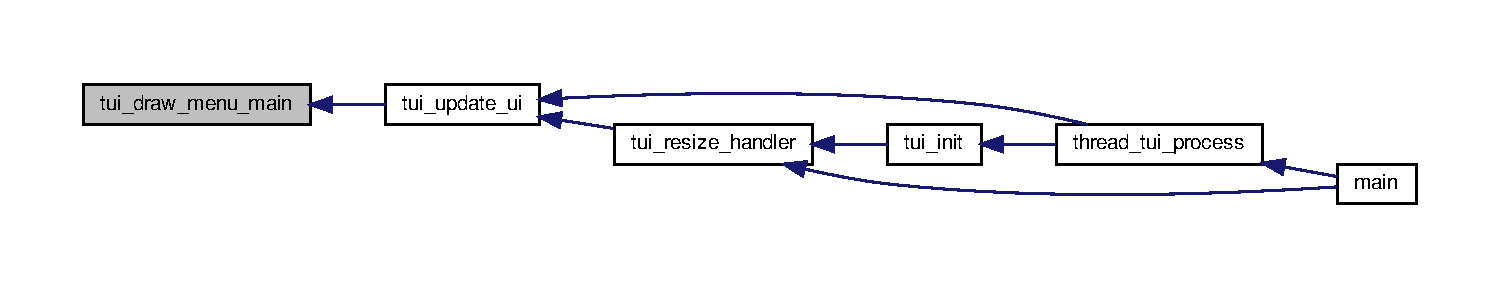
\includegraphics[width=350pt]{tui_8c_abb0281366396994ce0f56021e9927672_icgraph}
\end{center}
\end{figure}
\mbox{\Hypertarget{tui_8c_a54881c6b451cb64d9885435dea38f0e3}\label{tui_8c_a54881c6b451cb64d9885435dea38f0e3}} 
\index{tui.\+c@{tui.\+c}!tui\+\_\+draw\+\_\+panel\+\_\+info@{tui\+\_\+draw\+\_\+panel\+\_\+info}}
\index{tui\+\_\+draw\+\_\+panel\+\_\+info@{tui\+\_\+draw\+\_\+panel\+\_\+info}!tui.\+c@{tui.\+c}}
\subsubsection{\texorpdfstring{tui\+\_\+draw\+\_\+panel\+\_\+info()}{tui\_draw\_panel\_info()}}
{\footnotesize\ttfamily void tui\+\_\+draw\+\_\+panel\+\_\+info (\begin{DoxyParamCaption}{ }\end{DoxyParamCaption})}

Here is the caller graph for this function\+:\nopagebreak
\begin{figure}[H]
\begin{center}
\leavevmode
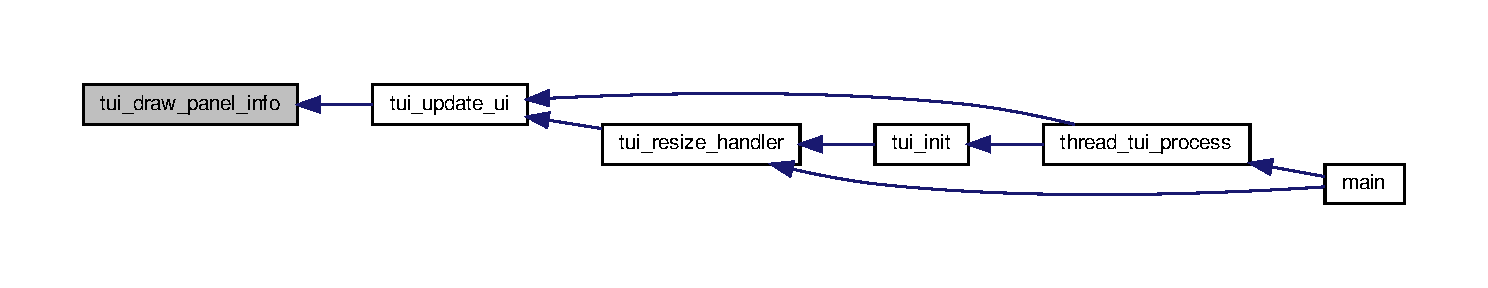
\includegraphics[width=350pt]{tui_8c_a54881c6b451cb64d9885435dea38f0e3_icgraph}
\end{center}
\end{figure}
\mbox{\Hypertarget{tui_8c_a846538693ed09ad0b9d77bac54f670e6}\label{tui_8c_a846538693ed09ad0b9d77bac54f670e6}} 
\index{tui.\+c@{tui.\+c}!tui\+\_\+draw\+\_\+panel\+\_\+notify\+\_\+exit@{tui\+\_\+draw\+\_\+panel\+\_\+notify\+\_\+exit}}
\index{tui\+\_\+draw\+\_\+panel\+\_\+notify\+\_\+exit@{tui\+\_\+draw\+\_\+panel\+\_\+notify\+\_\+exit}!tui.\+c@{tui.\+c}}
\subsubsection{\texorpdfstring{tui\+\_\+draw\+\_\+panel\+\_\+notify\+\_\+exit()}{tui\_draw\_panel\_notify\_exit()}}
{\footnotesize\ttfamily void tui\+\_\+draw\+\_\+panel\+\_\+notify\+\_\+exit (\begin{DoxyParamCaption}{ }\end{DoxyParamCaption})}

Here is the caller graph for this function\+:\nopagebreak
\begin{figure}[H]
\begin{center}
\leavevmode
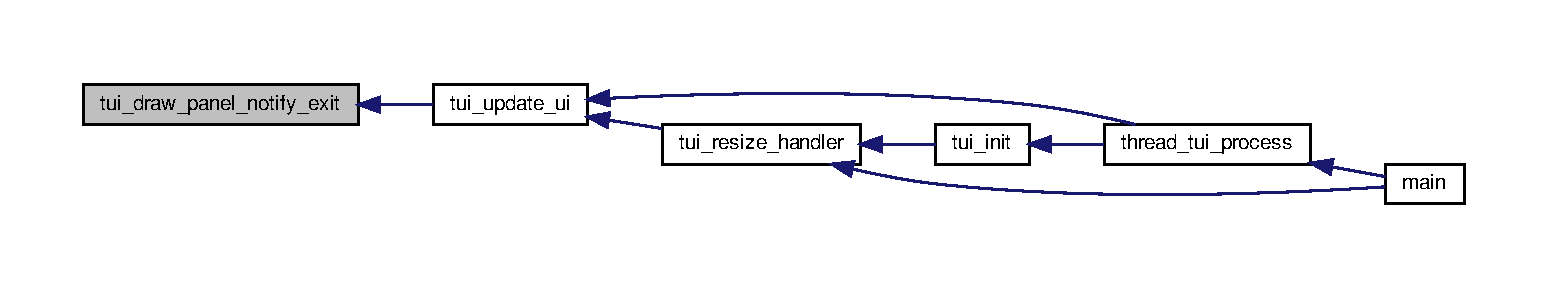
\includegraphics[width=350pt]{tui_8c_a846538693ed09ad0b9d77bac54f670e6_icgraph}
\end{center}
\end{figure}
\mbox{\Hypertarget{tui_8c_a7bda53a19c8ccfc47315be86386127c8}\label{tui_8c_a7bda53a19c8ccfc47315be86386127c8}} 
\index{tui.\+c@{tui.\+c}!tui\+\_\+draw\+\_\+panel\+\_\+option\+\_\+menu@{tui\+\_\+draw\+\_\+panel\+\_\+option\+\_\+menu}}
\index{tui\+\_\+draw\+\_\+panel\+\_\+option\+\_\+menu@{tui\+\_\+draw\+\_\+panel\+\_\+option\+\_\+menu}!tui.\+c@{tui.\+c}}
\subsubsection{\texorpdfstring{tui\+\_\+draw\+\_\+panel\+\_\+option\+\_\+menu()}{tui\_draw\_panel\_option\_menu()}}
{\footnotesize\ttfamily void tui\+\_\+draw\+\_\+panel\+\_\+option\+\_\+menu (\begin{DoxyParamCaption}{ }\end{DoxyParamCaption})}

Here is the caller graph for this function\+:\nopagebreak
\begin{figure}[H]
\begin{center}
\leavevmode
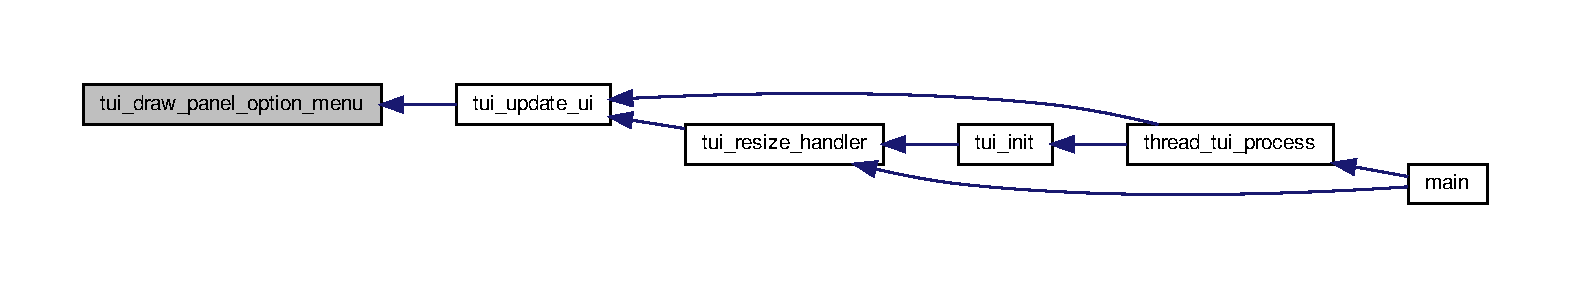
\includegraphics[width=350pt]{tui_8c_a7bda53a19c8ccfc47315be86386127c8_icgraph}
\end{center}
\end{figure}
\mbox{\Hypertarget{tui_8c_abd6db3f802be383d230bc2249d3a6652}\label{tui_8c_abd6db3f802be383d230bc2249d3a6652}} 
\index{tui.\+c@{tui.\+c}!tui\+\_\+draw\+\_\+panel\+\_\+schem\+\_\+viewer@{tui\+\_\+draw\+\_\+panel\+\_\+schem\+\_\+viewer}}
\index{tui\+\_\+draw\+\_\+panel\+\_\+schem\+\_\+viewer@{tui\+\_\+draw\+\_\+panel\+\_\+schem\+\_\+viewer}!tui.\+c@{tui.\+c}}
\subsubsection{\texorpdfstring{tui\+\_\+draw\+\_\+panel\+\_\+schem\+\_\+viewer()}{tui\_draw\_panel\_schem\_viewer()}}
{\footnotesize\ttfamily void tui\+\_\+draw\+\_\+panel\+\_\+schem\+\_\+viewer (\begin{DoxyParamCaption}{ }\end{DoxyParamCaption})}

Here is the caller graph for this function\+:\nopagebreak
\begin{figure}[H]
\begin{center}
\leavevmode
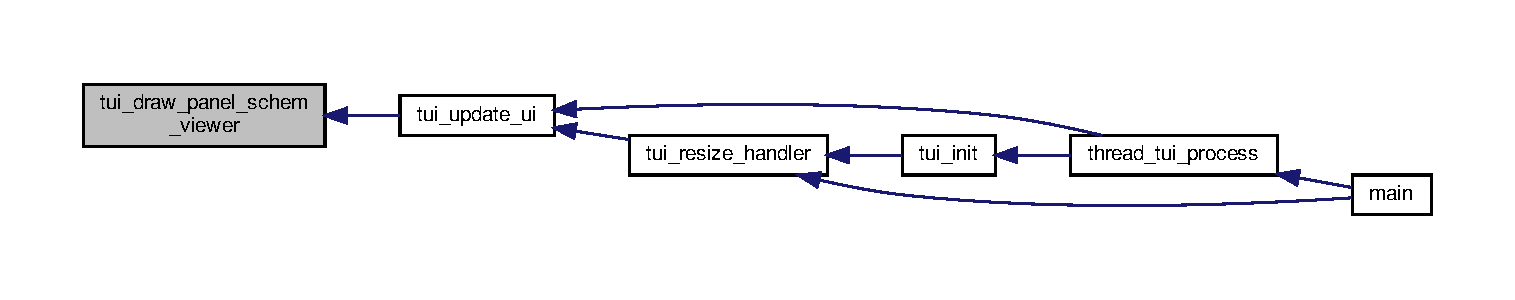
\includegraphics[width=350pt]{tui_8c_abd6db3f802be383d230bc2249d3a6652_icgraph}
\end{center}
\end{figure}
\mbox{\Hypertarget{tui_8c_aa0edec0264532eb82d3b5cde3c11160e}\label{tui_8c_aa0edec0264532eb82d3b5cde3c11160e}} 
\index{tui.\+c@{tui.\+c}!tui\+\_\+draw\+\_\+panel\+\_\+src\+\_\+browser@{tui\+\_\+draw\+\_\+panel\+\_\+src\+\_\+browser}}
\index{tui\+\_\+draw\+\_\+panel\+\_\+src\+\_\+browser@{tui\+\_\+draw\+\_\+panel\+\_\+src\+\_\+browser}!tui.\+c@{tui.\+c}}
\subsubsection{\texorpdfstring{tui\+\_\+draw\+\_\+panel\+\_\+src\+\_\+browser()}{tui\_draw\_panel\_src\_browser()}}
{\footnotesize\ttfamily void tui\+\_\+draw\+\_\+panel\+\_\+src\+\_\+browser (\begin{DoxyParamCaption}{ }\end{DoxyParamCaption})}

Here is the caller graph for this function\+:\nopagebreak
\begin{figure}[H]
\begin{center}
\leavevmode
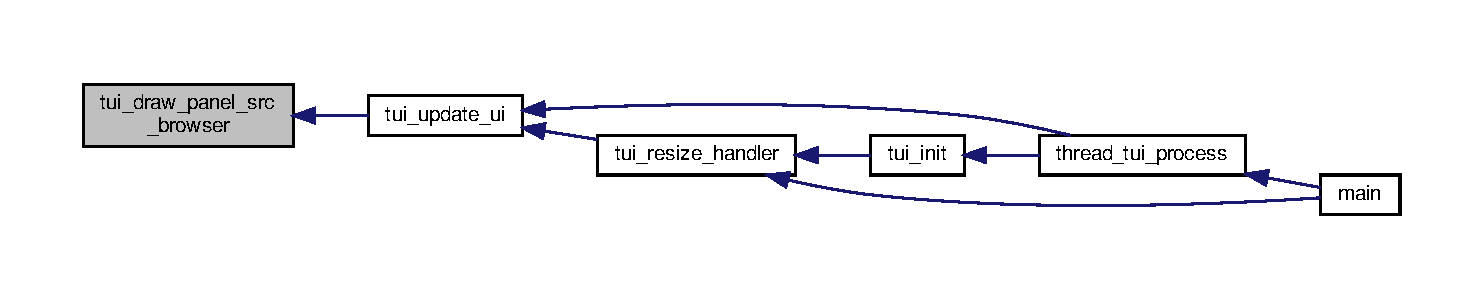
\includegraphics[width=350pt]{tui_8c_aa0edec0264532eb82d3b5cde3c11160e_icgraph}
\end{center}
\end{figure}
\mbox{\Hypertarget{tui_8c_a1950cd06f7947f91941838bf3ed64f7f}\label{tui_8c_a1950cd06f7947f91941838bf3ed64f7f}} 
\index{tui.\+c@{tui.\+c}!tui\+\_\+draw\+\_\+window\+\_\+base@{tui\+\_\+draw\+\_\+window\+\_\+base}}
\index{tui\+\_\+draw\+\_\+window\+\_\+base@{tui\+\_\+draw\+\_\+window\+\_\+base}!tui.\+c@{tui.\+c}}
\subsubsection{\texorpdfstring{tui\+\_\+draw\+\_\+window\+\_\+base()}{tui\_draw\_window\_base()}}
{\footnotesize\ttfamily void tui\+\_\+draw\+\_\+window\+\_\+base (\begin{DoxyParamCaption}{ }\end{DoxyParamCaption})}

Here is the caller graph for this function\+:\nopagebreak
\begin{figure}[H]
\begin{center}
\leavevmode
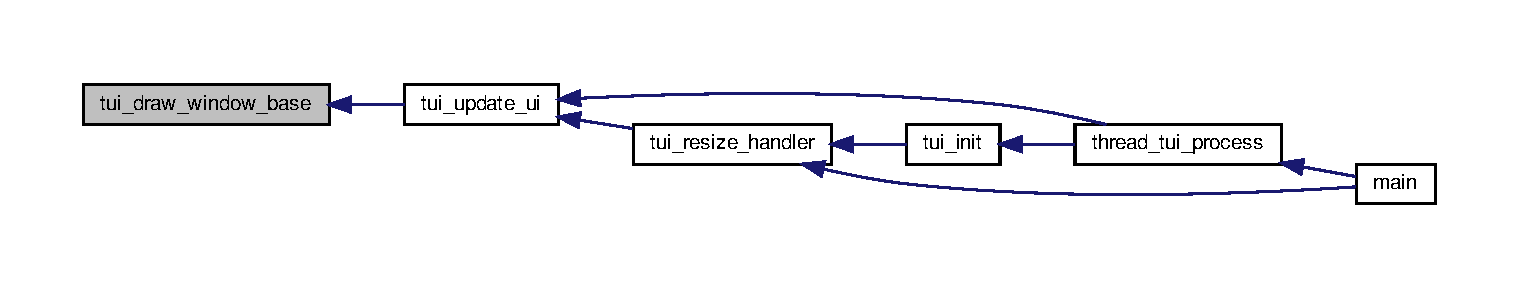
\includegraphics[width=350pt]{tui_8c_a1950cd06f7947f91941838bf3ed64f7f_icgraph}
\end{center}
\end{figure}
\mbox{\Hypertarget{tui_8c_a50220f3c4859104f84b4b5b06f6074fe}\label{tui_8c_a50220f3c4859104f84b4b5b06f6074fe}} 
\index{tui.\+c@{tui.\+c}!tui\+\_\+handle\+\_\+input@{tui\+\_\+handle\+\_\+input}}
\index{tui\+\_\+handle\+\_\+input@{tui\+\_\+handle\+\_\+input}!tui.\+c@{tui.\+c}}
\subsubsection{\texorpdfstring{tui\+\_\+handle\+\_\+input()}{tui\_handle\_input()}}
{\footnotesize\ttfamily int tui\+\_\+handle\+\_\+input (\begin{DoxyParamCaption}{ }\end{DoxyParamCaption})}

Here is the caller graph for this function\+:\nopagebreak
\begin{figure}[H]
\begin{center}
\leavevmode
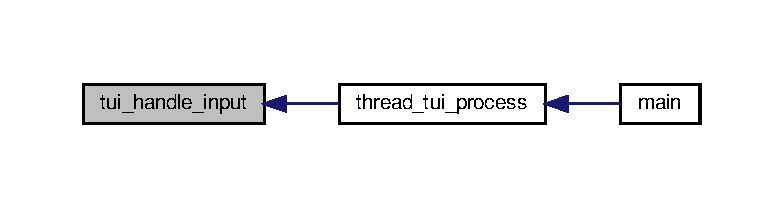
\includegraphics[width=350pt]{tui_8c_a50220f3c4859104f84b4b5b06f6074fe_icgraph}
\end{center}
\end{figure}
\mbox{\Hypertarget{tui_8c_a273e0f27732fe6b4c2644927a14e9428}\label{tui_8c_a273e0f27732fe6b4c2644927a14e9428}} 
\index{tui.\+c@{tui.\+c}!tui\+\_\+init@{tui\+\_\+init}}
\index{tui\+\_\+init@{tui\+\_\+init}!tui.\+c@{tui.\+c}}
\subsubsection{\texorpdfstring{tui\+\_\+init()}{tui\_init()}}
{\footnotesize\ttfamily void tui\+\_\+init (\begin{DoxyParamCaption}{ }\end{DoxyParamCaption})}



H\+I\+FN Initializes the UI interface, and panels. 

Here is the call graph for this function\+:\nopagebreak
\begin{figure}[H]
\begin{center}
\leavevmode
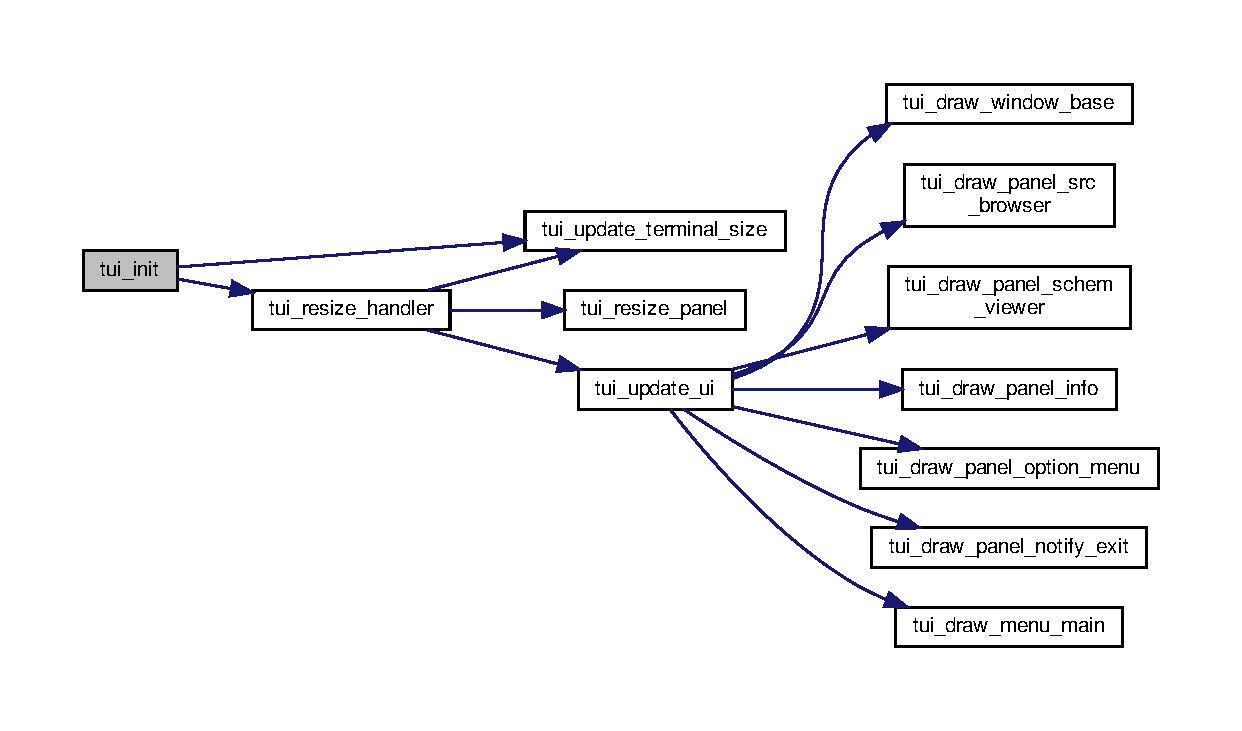
\includegraphics[width=350pt]{tui_8c_a273e0f27732fe6b4c2644927a14e9428_cgraph}
\end{center}
\end{figure}
Here is the caller graph for this function\+:\nopagebreak
\begin{figure}[H]
\begin{center}
\leavevmode
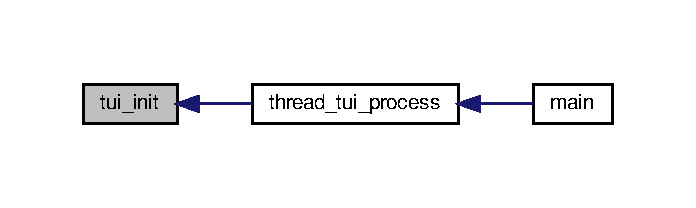
\includegraphics[width=334pt]{tui_8c_a273e0f27732fe6b4c2644927a14e9428_icgraph}
\end{center}
\end{figure}
\mbox{\Hypertarget{tui_8c_a933a448d1adf3cac78fd3a75f729a521}\label{tui_8c_a933a448d1adf3cac78fd3a75f729a521}} 
\index{tui.\+c@{tui.\+c}!tui\+\_\+resize\+\_\+handler@{tui\+\_\+resize\+\_\+handler}}
\index{tui\+\_\+resize\+\_\+handler@{tui\+\_\+resize\+\_\+handler}!tui.\+c@{tui.\+c}}
\subsubsection{\texorpdfstring{tui\+\_\+resize\+\_\+handler()}{tui\_resize\_handler()}}
{\footnotesize\ttfamily void tui\+\_\+resize\+\_\+handler (\begin{DoxyParamCaption}\item[{int}]{sig }\end{DoxyParamCaption})}

Here is the call graph for this function\+:\nopagebreak
\begin{figure}[H]
\begin{center}
\leavevmode
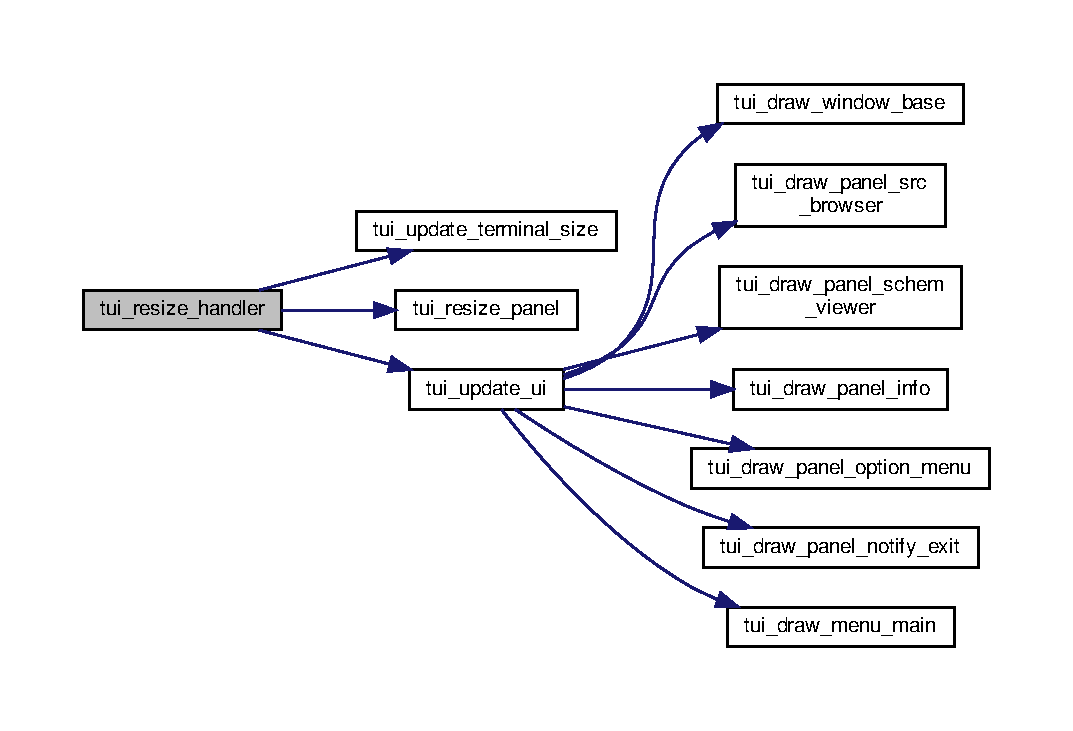
\includegraphics[width=350pt]{tui_8c_a933a448d1adf3cac78fd3a75f729a521_cgraph}
\end{center}
\end{figure}
Here is the caller graph for this function\+:\nopagebreak
\begin{figure}[H]
\begin{center}
\leavevmode
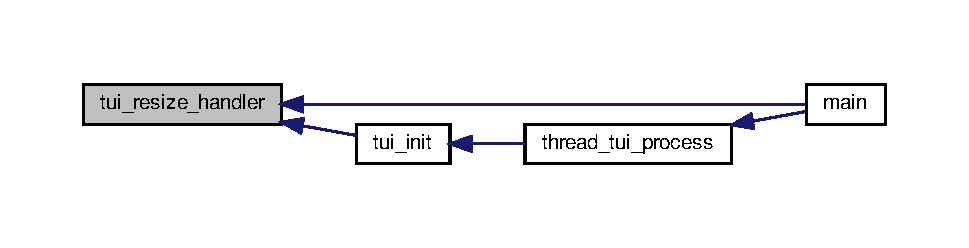
\includegraphics[width=350pt]{tui_8c_a933a448d1adf3cac78fd3a75f729a521_icgraph}
\end{center}
\end{figure}
\mbox{\Hypertarget{tui_8c_ae858f3690f75bd2604de07d3c53f7f8c}\label{tui_8c_ae858f3690f75bd2604de07d3c53f7f8c}} 
\index{tui.\+c@{tui.\+c}!tui\+\_\+resize\+\_\+panel@{tui\+\_\+resize\+\_\+panel}}
\index{tui\+\_\+resize\+\_\+panel@{tui\+\_\+resize\+\_\+panel}!tui.\+c@{tui.\+c}}
\subsubsection{\texorpdfstring{tui\+\_\+resize\+\_\+panel()}{tui\_resize\_panel()}}
{\footnotesize\ttfamily void tui\+\_\+resize\+\_\+panel (\begin{DoxyParamCaption}\item[{P\+A\+N\+EL $\ast$}]{panel,  }\item[{int}]{rows,  }\item[{int}]{cols,  }\item[{int}]{start\+\_\+y,  }\item[{int}]{start\+\_\+x }\end{DoxyParamCaption})}

Here is the caller graph for this function\+:\nopagebreak
\begin{figure}[H]
\begin{center}
\leavevmode
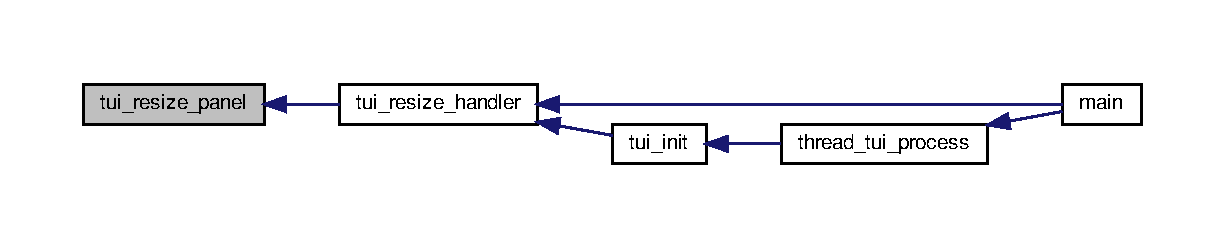
\includegraphics[width=350pt]{tui_8c_ae858f3690f75bd2604de07d3c53f7f8c_icgraph}
\end{center}
\end{figure}
\mbox{\Hypertarget{tui_8c_aad57a653d5bc57141d3bb73b4a29b9e9}\label{tui_8c_aad57a653d5bc57141d3bb73b4a29b9e9}} 
\index{tui.\+c@{tui.\+c}!tui\+\_\+stop@{tui\+\_\+stop}}
\index{tui\+\_\+stop@{tui\+\_\+stop}!tui.\+c@{tui.\+c}}
\subsubsection{\texorpdfstring{tui\+\_\+stop()}{tui\_stop()}}
{\footnotesize\ttfamily void tui\+\_\+stop (\begin{DoxyParamCaption}{ }\end{DoxyParamCaption})}



H\+I\+FN Deinitializes the UI interface and panels. 

Here is the caller graph for this function\+:\nopagebreak
\begin{figure}[H]
\begin{center}
\leavevmode
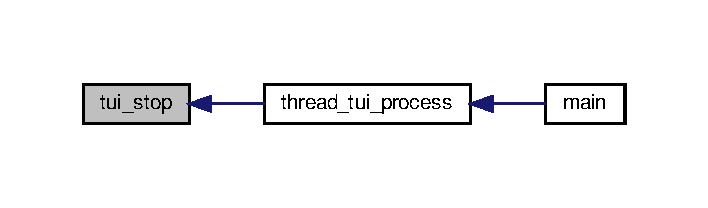
\includegraphics[width=340pt]{tui_8c_aad57a653d5bc57141d3bb73b4a29b9e9_icgraph}
\end{center}
\end{figure}
\mbox{\Hypertarget{tui_8c_a0b806bb14243bf0259f03648dc23f9be}\label{tui_8c_a0b806bb14243bf0259f03648dc23f9be}} 
\index{tui.\+c@{tui.\+c}!tui\+\_\+update\+\_\+terminal\+\_\+size@{tui\+\_\+update\+\_\+terminal\+\_\+size}}
\index{tui\+\_\+update\+\_\+terminal\+\_\+size@{tui\+\_\+update\+\_\+terminal\+\_\+size}!tui.\+c@{tui.\+c}}
\subsubsection{\texorpdfstring{tui\+\_\+update\+\_\+terminal\+\_\+size()}{tui\_update\_terminal\_size()}}
{\footnotesize\ttfamily void tui\+\_\+update\+\_\+terminal\+\_\+size (\begin{DoxyParamCaption}{ }\end{DoxyParamCaption})}

Here is the caller graph for this function\+:\nopagebreak
\begin{figure}[H]
\begin{center}
\leavevmode
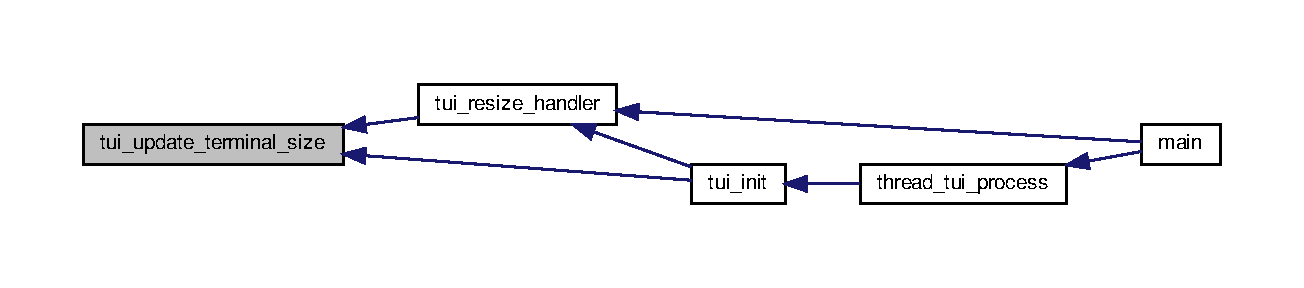
\includegraphics[width=350pt]{tui_8c_a0b806bb14243bf0259f03648dc23f9be_icgraph}
\end{center}
\end{figure}
\mbox{\Hypertarget{tui_8c_a37ebe23d01d303deb649c64afb7b68ea}\label{tui_8c_a37ebe23d01d303deb649c64afb7b68ea}} 
\index{tui.\+c@{tui.\+c}!tui\+\_\+update\+\_\+ui@{tui\+\_\+update\+\_\+ui}}
\index{tui\+\_\+update\+\_\+ui@{tui\+\_\+update\+\_\+ui}!tui.\+c@{tui.\+c}}
\subsubsection{\texorpdfstring{tui\+\_\+update\+\_\+ui()}{tui\_update\_ui()}}
{\footnotesize\ttfamily void tui\+\_\+update\+\_\+ui (\begin{DoxyParamCaption}{ }\end{DoxyParamCaption})}

Here is the call graph for this function\+:\nopagebreak
\begin{figure}[H]
\begin{center}
\leavevmode
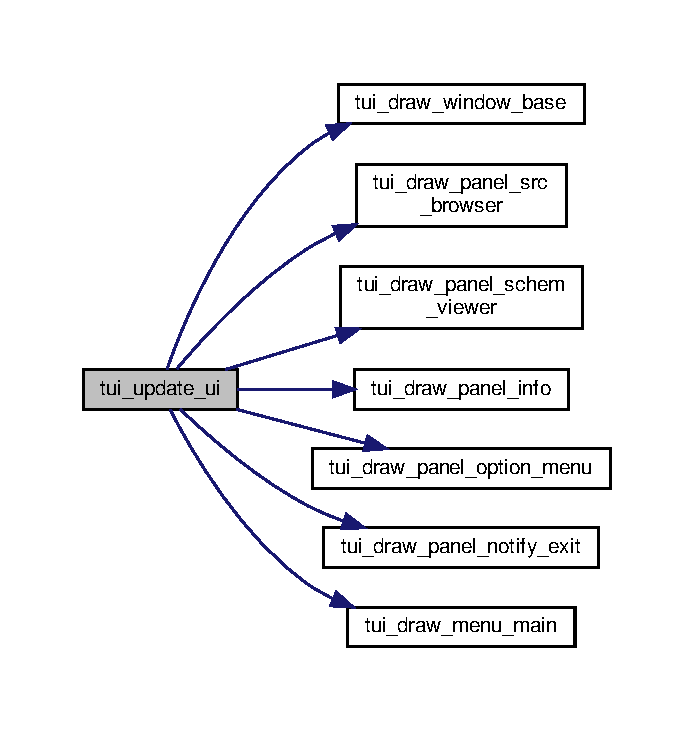
\includegraphics[width=333pt]{tui_8c_a37ebe23d01d303deb649c64afb7b68ea_cgraph}
\end{center}
\end{figure}
Here is the caller graph for this function\+:\nopagebreak
\begin{figure}[H]
\begin{center}
\leavevmode
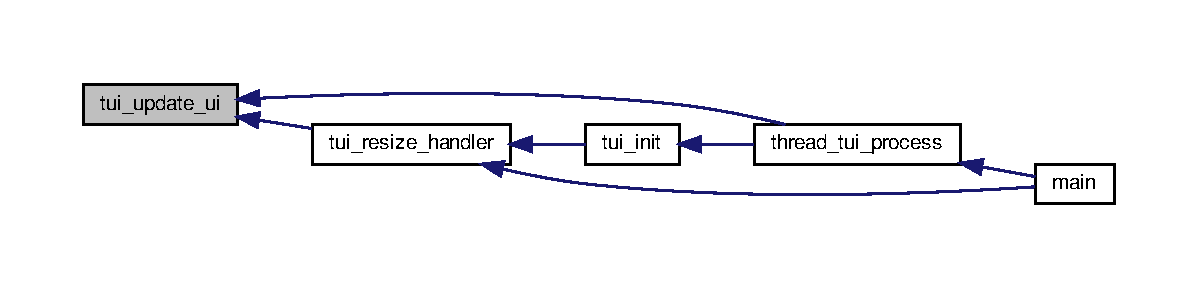
\includegraphics[width=350pt]{tui_8c_a37ebe23d01d303deb649c64afb7b68ea_icgraph}
\end{center}
\end{figure}


\subsection{Variable Documentation}
\mbox{\Hypertarget{tui_8c_a572464641a2c1bc384664c3eccdedb37}\label{tui_8c_a572464641a2c1bc384664c3eccdedb37}} 
\index{tui.\+c@{tui.\+c}!panel\+\_\+info@{panel\+\_\+info}}
\index{panel\+\_\+info@{panel\+\_\+info}!tui.\+c@{tui.\+c}}
\subsubsection{\texorpdfstring{panel\+\_\+info}{panel\_info}}
{\footnotesize\ttfamily P\+A\+N\+EL$\ast$ panel\+\_\+info}

\mbox{\Hypertarget{tui_8c_a93d0ddb825e58ca3d110e91a15985ddc}\label{tui_8c_a93d0ddb825e58ca3d110e91a15985ddc}} 
\index{tui.\+c@{tui.\+c}!panel\+\_\+notify\+\_\+exit@{panel\+\_\+notify\+\_\+exit}}
\index{panel\+\_\+notify\+\_\+exit@{panel\+\_\+notify\+\_\+exit}!tui.\+c@{tui.\+c}}
\subsubsection{\texorpdfstring{panel\+\_\+notify\+\_\+exit}{panel\_notify\_exit}}
{\footnotesize\ttfamily P\+A\+N\+EL$\ast$ panel\+\_\+notify\+\_\+exit}

\mbox{\Hypertarget{tui_8c_aba18483ea17ea7d407bcda3d84dc038a}\label{tui_8c_aba18483ea17ea7d407bcda3d84dc038a}} 
\index{tui.\+c@{tui.\+c}!panel\+\_\+option\+\_\+menu@{panel\+\_\+option\+\_\+menu}}
\index{panel\+\_\+option\+\_\+menu@{panel\+\_\+option\+\_\+menu}!tui.\+c@{tui.\+c}}
\subsubsection{\texorpdfstring{panel\+\_\+option\+\_\+menu}{panel\_option\_menu}}
{\footnotesize\ttfamily P\+A\+N\+EL$\ast$ panel\+\_\+option\+\_\+menu}

\mbox{\Hypertarget{tui_8c_a9493ac7691dab866ea00b0cbefb084dd}\label{tui_8c_a9493ac7691dab866ea00b0cbefb084dd}} 
\index{tui.\+c@{tui.\+c}!panel\+\_\+schem\+\_\+viewer@{panel\+\_\+schem\+\_\+viewer}}
\index{panel\+\_\+schem\+\_\+viewer@{panel\+\_\+schem\+\_\+viewer}!tui.\+c@{tui.\+c}}
\subsubsection{\texorpdfstring{panel\+\_\+schem\+\_\+viewer}{panel\_schem\_viewer}}
{\footnotesize\ttfamily P\+A\+N\+EL$\ast$ panel\+\_\+schem\+\_\+viewer}

\mbox{\Hypertarget{tui_8c_a587539204549f96820fe58427e2e28e9}\label{tui_8c_a587539204549f96820fe58427e2e28e9}} 
\index{tui.\+c@{tui.\+c}!panel\+\_\+src\+\_\+browser@{panel\+\_\+src\+\_\+browser}}
\index{panel\+\_\+src\+\_\+browser@{panel\+\_\+src\+\_\+browser}!tui.\+c@{tui.\+c}}
\subsubsection{\texorpdfstring{panel\+\_\+src\+\_\+browser}{panel\_src\_browser}}
{\footnotesize\ttfamily P\+A\+N\+EL$\ast$ panel\+\_\+src\+\_\+browser}

\mbox{\Hypertarget{tui_8c_a3992660c8f7cbec313e690e6b9f310da}\label{tui_8c_a3992660c8f7cbec313e690e6b9f310da}} 
\index{tui.\+c@{tui.\+c}!window\+\_\+base@{window\+\_\+base}}
\index{window\+\_\+base@{window\+\_\+base}!tui.\+c@{tui.\+c}}
\subsubsection{\texorpdfstring{window\+\_\+base}{window\_base}}
{\footnotesize\ttfamily W\+I\+N\+D\+OW$\ast$ window\+\_\+base}


%--- End generated contents ---

% Index
\backmatter
\newpage
\phantomsection
\clearemptydoublepage
\addcontentsline{toc}{chapter}{Index}
\printindex

\end{document}
